\chapter{La modélisation du carrefour}

% Intro du chapitre : ma modélisation est basée sur OSM donc je décris ce que contient OSM

Le carrefour peut être un espace d'interaction entre piétons et véhicules. Dans le cas où il permet à un piéton de le franchir, la signalisation permet alternativement aux flux des piétons ou des voitures de le traverser en sécurité. Pour une \gls{pcdv}, cette traversée peut être complexe en raison de la variabilité et l'hétérogénéité des configurations, du nombre de voies présentes, et des équipements de contrôle du trafic et d'accessibilité. Dans ce chapitre, nous présentons l'architecture du carrefour du point de vue d'une personne concernée, puis nous analysons au regard des besoins évoqués la manière dont ces données sont représentées dans la base de données \gls{osm}. Enfin, nous proposons une représentation objet de la donnée \gls{osm} que nous appliquons à une modélisation du carrefour orientée sur l'accessibilité.

% Un "état de l'art" à la JLZ pour chaque sous-partie : une vue précise du carrefour, de son infrastructure et des éléments d'accessibilité qui le compose.
% Penser le carrefour du point de vue du piéton sous la forme d'un graphe 

\section{La structure globale du carrefour}

% Pour définir les éléments de mon modèle, j'ai utilisé des méthodo de travail : je suis allé interroger des professionnels, etc. Mentionner le fait d'être allé rencontrer des personnes du CRDV, autres professionnels.

Un carrefour, tel que défini par le dictionnaire Larousse, est un \pquote{lieu où se croisent plusieurs rues ou plusieurs routes, généralement aménagé en vue d'éviter les risques de collision, et parfois d'améliorer le débit}. Une particularité concernant nos travaux est que le carrefour nous intéresse du point de vue du piéton, et notamment du piéton concerné par la déficience visuelle, dont les spécificités doivent être prise en compte dans la définition d'un carrefour tel que nous le concevons. Lors des travaux préliminaires à ce mémoire, nous avons interrogé des personnes concernées et professionnels du \gls{crdv} de Clermont-Ferrand pour établir cette définition. Pour ces dernières, la limite d'un carrefour correspond à l'étendue de ce qu'une personne peut entendre. Bien qu'il existe des travaux de modélisation accoustique\comment{Ajouter une référence} orientés notamment sur la propagation du bruit, cette approche nous semble difficile à généraliser dans un premier temps. Nous avons donc choisi de nous concentrer tout d'abord sur la structure du carrefour du point de vue du piéton, en en proposant une représentation sous forme de graphe, puis en s'intéressant aux élements d'accessibilité spécifiques à la mobilité des \glspl{pcdv}.


% \begin{figure}
%     \centering
%     \resizebox{15cm}{!}{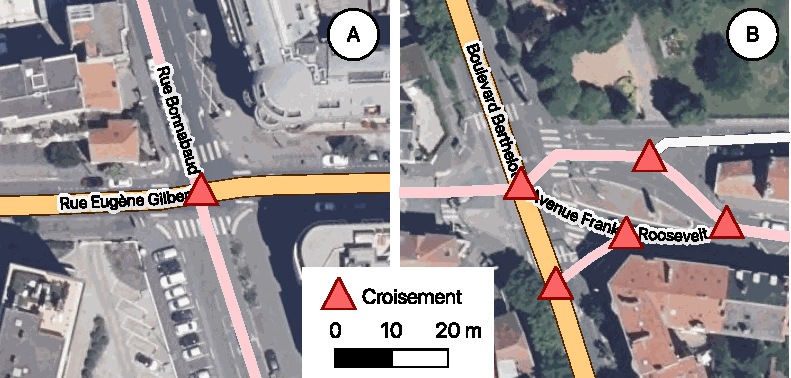
\includegraphics{images/modelisation/mod_simple_complexe.pdf}}
%     \caption[La délimitation du carrefour]{Un carrefour peut être difficile à délimiter quand il ne s'agit pas d'un unique croisement. La délimitation du carrefour B dépend de la définition que l'on souhaite prendre du carrefour, et peut être en réalité composé de plusieurs sous-carrefours. Sources : Orthophotographie CRAIG, Contributeurs OpenStreetMap.}
%     \label{fig:modelisation_simplecomplexe}
% \end{figure}

% Structure en branches
% On se place du point de vue du piéton, ce sont les trottoirs qui comptent.

\subsection{Le graphe du carrefour du point de vue d'un piéton}

\label{sec:modelisation_definitions}

Pour modéliser le carrefour du point de vue d'un piéton, nous avons choisi de nous reposer sur une approche graphe afin de le définir et de le délimiter dans un réseau routier. Les définitions suivantes en définissent la structure :

\begin{definition}
    On appelle \textbf{couverture} d'un graphe $G_0 = (V_0,E_0)$ et plongé dans le plan un ensemble de sous-graphes $\mathcal{G_0}$ tels que:
    \begin{itemize}
        \item Si $G_1=(V_1, E_1) \in \mathcal{G_0}$ et $G_2=(V_2, E_2) \in \mathcal{G_p}$, alors $E_1 \cap E_2 = \emptyset$
        \item $\forall e \in E_p$, $\exists!~G_1=(V_1, E_1) \in \mathcal{G_p}$ tel que $e \in E_1$
    \end{itemize}
    
    Dans la suite, on appelle $\mathcal{G}_p$ une couverture du graphe piéton, et $\mathcal{G}_r$ une couverture du graphe routier.
    
    Dans la suite, on dira que deux sous-graphes sont \textbf{connectés} s'ils partagent au moins un sommet en commun.
\end{definition}

\begin{definition}
    On défini un \textbf{graphe multimodal} comme un graphe $G = (V,E)$ plongé dans le plan et muni d'une couverture $\{G_r=(V_r, E_r), G_p = (V_p, E_p)\}$ composée d'un \textbf{graphe routier} $G_r$ et d'un \textbf{graphe piéton} $G_p$.

    Dans la suite, on note $G = (V,E)$ un graphe multimodal sur lequel on défini les autres ensembles et propriétés.
\end{definition}

\noindent
Remarque: l'intersection entre $V_r$ et $V_p$ peut ne pas être vide.

\begin{definition}
    Soient $G_1=(V_1, E_1)$ et $G_2=(V_2, E_2)$ deux sous-graphes de $G=(V, E)$.
    
    On appelle \textbf{fonction d'association} $f: E_1 \rightarrow E_2$ toute fonction qui à chaque arête de $G_1$ associe une arête de $G_2$.
\end{definition}

\begin{definition}
    Alors on appelle \textbf{trottoir} tout $G_t = (V_t, E_t)\in \mathcal{G}_p$ sous-graphe du graphe piéton muni d'une fonction d'association $f_t: G_t \rightarrow G_r$ projetant les arêtes de $G_t$ dans le graphe routier. Cette fonction $f_t$ est appelée \textbf{fonction d'adjacence} du trottoir $G_t$.

    On note $\mathcal{G}_t$ l'ensemble des trottoirs.
\end{definition}

\begin{definition}
    Étant donné une couverture $\mathcal{G}_p$ d'un graphe piéton $G_p$, un ensemble de fonctions d'adjacence est dit \textbf{un ensemble de trottoirs couvrants} s'il n'existe pas de sommet $v \in G_p$ appartenant à plus d'un trottoir.
\end{definition}

\noindent
Exemple: couverture d'un graphe piéton qui n'est pas un ensemble de trottoirs couvrants (voir Figure \ref{fig:mod_ex_trottoirs_couvrants}).

\begin{figure}
    \centering
    
\includegraphics{images/placeholder.jpg}
    \caption{Ces deux trottoirs ne sont pas couvrants car ils possèdent un noeud en commun.}
    \label{fig:mod_ex_trottoirs_couvrants}
\end{figure}

\begin{definition}
    On appelle \textbf{chemin} un graphe $G_{ch} = (V_{ch}, E_{ch})$ tel que $V_{ch}=\{p_1,p_2,\dots,p_n\}$ et $E_{ch}=\{\{p_1,p_2\},\{p_2,p_3\},\dots,\{p_{n-1},p_n\}\}$.
\end{definition}

\begin{definition}
    Un \textbf{passage piéton} $G_{pp} = (V_{pp}, E_{pp}) \in \mathcal{G}_p$ est un chemin $(p_1, p_2,\dots, p_n)$ tel que:

    \begin{itemize}
        \item $p_2, p_3, \dots, p_{n-1}$ sont inclus dans le graphe routier
        \item $p_2, p_3, \dots, p_{n-1}$ n'appartiennent pas à un trottoir
        \item $p_1$ et $p_n$ appartiennent chacun à un trottoir
    \end{itemize}
\end{definition}

\begin{definition}
    Une couverture $\mathcal{G}_r$ d'un réseau routier est dite \textbf{couverture routière complète} si et seulement si elle est composée d'une union disjointe de \textbf{coeurs de carrefours} $\mathcal{G}_c \subset \mathcal{G}_r$ et de \textbf{branches} $\mathcal{G}_b \subset \mathcal{G}_r$ tels que:

    \begin{itemize}
        \item $\mathcal{G}_c \neq \emptyset$ 
        \item Deux coeurs de carrefour ne sont pas connectés
        \item Chaque branche est connectée à un ou deux coeurs de carrefour
        \item Un coeur de carrefour est au minimum connecté à deux branches distinctes
    \end{itemize}
    \label{def:modelisation_couverture_routiere_complète}
\end{definition}

\noindent
Remarque: un cœur de carrefour ne peut pas être un chemin.

\noindent
Exemples:
\begin{itemize}
    \item Une couverture routière qui n'est pas complète (voir Figure \ref{fig:mod_ex_couverture_routiere_incomplete})
    \item Une couverture routière de carrefour (voire Figure \ref{fig:mod_ex_couverture_routiere_carrefour})
    \item Une couverture routière à plusieurs carrefours, dites de quartier (voire Figure \ref{fig:mod_ex_couverture_routiere_quartier})
\end{itemize}

\begin{figure}
    \centering
    
\includegraphics{images/placeholder.jpg}
    \caption{Cette couverture routière est incomplète car \todo{}.}
    \label{fig:mod_ex_couverture_routiere_incomplete}
\end{figure}

\begin{figure}
    \centering
    
\includegraphics{images/placeholder.jpg}
    \caption{Cette couverture de carrefour montre \todo{}.}
    \label{fig:mod_ex_couverture_routiere_carrefour}
\end{figure}

\begin{figure}
    \centering
    
\includegraphics{images/placeholder.jpg}
    \caption{Une couverture de quartier comprend plusieurs carrefours.}
    \label{fig:mod_ex_couverture_routiere_quartier}
\end{figure}

\begin{definition}
    Une couverture $\mathcal{G}_p$ d'un réseau piéton est dite \textbf{couverture piétonne complète} si et seulement si elle est composée d'une union disjointe de trottoirs, de passages piétons, et d'\textbf{îlots} $\mathcal{G}_i \in \mathcal{G}_p$ tel qu'un îlot n'est connecté qu'à des passages piéton.
\end{definition}

\begin{definition}
    Une \textbf{traversée} $G_{t} = (V_{t}, E_{t}) \in \mathcal{G}_p$ est un chemin $(p_1, p_2,\dots, p_n)$ tel que:

    \begin{itemize}
        \item $p_1$ et $p_n$ appartiennent à un trottoir
        \item $p_2, p_3, \dots, p_{n-1}$ n'appartiennent pas à un trottoir
        \item $\forall e \in E_t$, $e$ appartient soit à un passage piéton, soit à un îlot
    \end{itemize}
\end{definition}

\begin{definition}
    Un \textbf{carrefour} est un graphe multimodal composé d'une couverture routière complète ne contenant qu'un seul cœur de carrefour, d'une couverture piétonne complète et d'un ensemble de traversées (voir Figure \ref{fig:mod_ex_graphe_carrefour}).
\end{definition}

\begin{figure}
    \centering
    
\includegraphics{images/placeholder.jpg}
    \caption{Le graphe multimodal d'un carrefour.}
    \label{fig:mod_ex_graphe_carrefour}
\end{figure}

% % Les branches du carrefour
% \begin{figure}
%     \centering
%     \resizebox{15cm}{!}{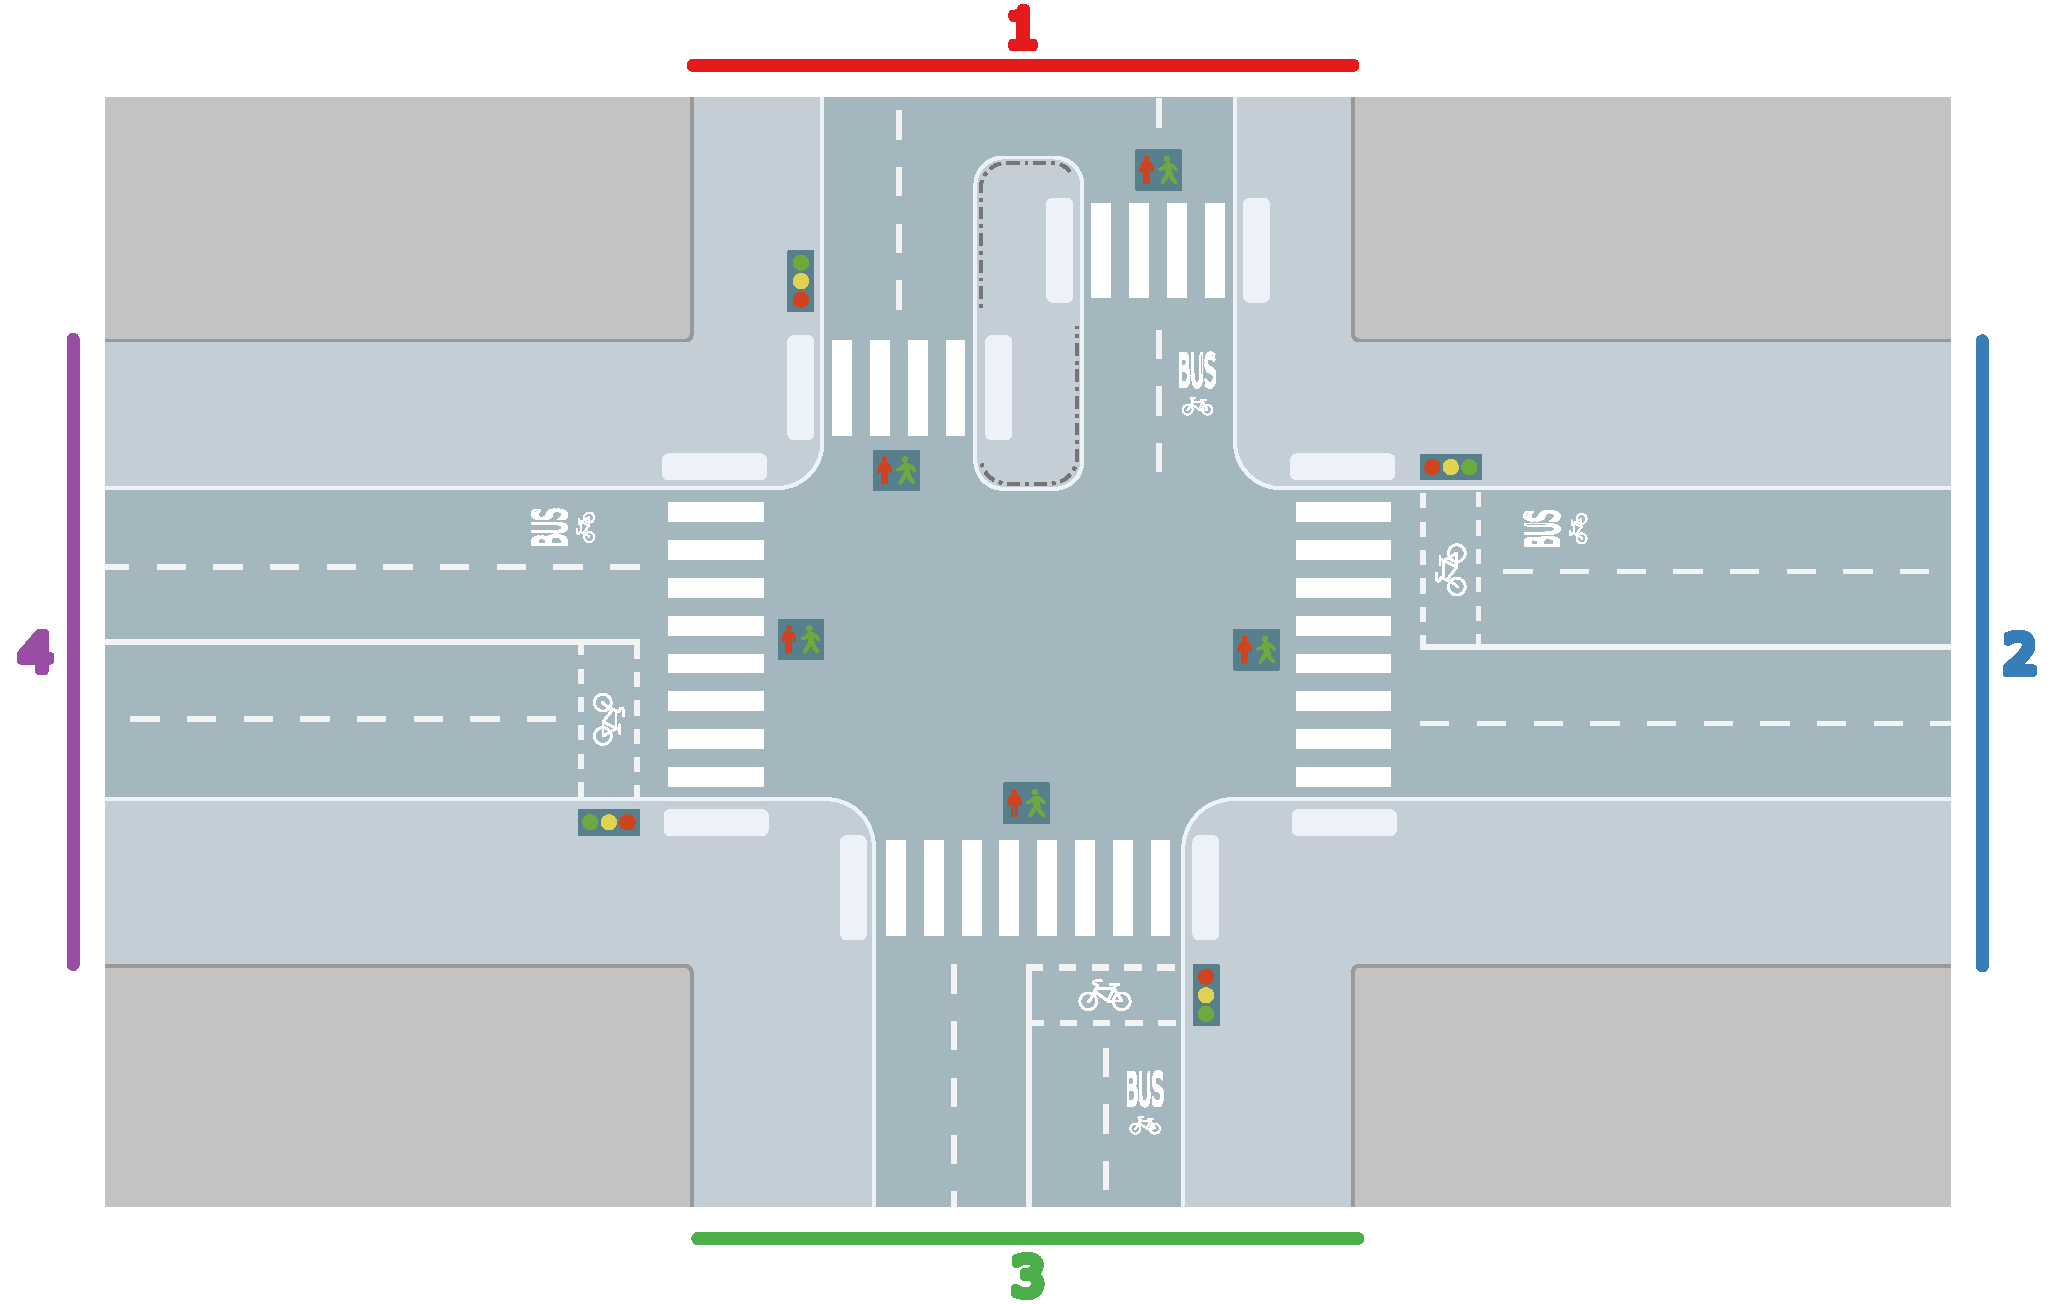
\includegraphics{images/modelisation/mod_branches.pdf}}
%     \caption{Ce carrefour composé de quatre branches est dit "en croix".}
%     \label{fig:modelisation_branche}
% \end{figure}

% % Une traversée du carrefour
% \begin{figure}
%     \centering
%     \resizebox{15cm}{!}{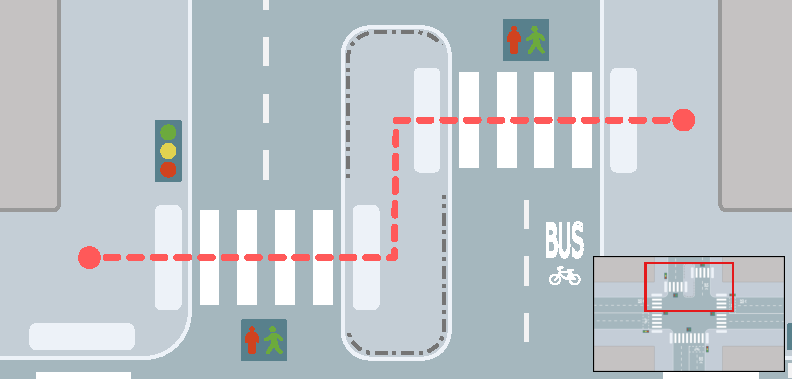
\includegraphics{images/modelisation/mod_traversee.pdf}}
%     \caption{Traversée d'une branche du carrefour.}
%     \label{fig:modelisation_traversee}
% \end{figure}

\subsection{Les repères au sein du carrefour}

\label{sec:mod_repere_carrefour}

Pour effectuer une traversée du carrefour en sécurité, il existe un certain nombre d'équipements d'accessibilité pouvant être mobilisés par une \gls{pcdv}. Ces équipements ont des rôles divers, comme permettre de repérer une traversée, ou d'y accéder par un nivellement adapté (dans le cas d'une \gls{pmr} par exemple). Pour répondre aux besoins des différents usagers, ces équipements font appel à des sens différents: l'ouïe pour les signaux sonores, le toucher pour les éléments tactiles, mais également la vue pour les potelets contrastés ou les passages piétons matérialisés par de la pleinture au sol qui peut être mobilisée par les \glspl{pcdv} présentant un résidu visuel. Plusieurs équipements pouvant être rencontrés sur un carrefour sont présentés au sein de la table \ref{tab:modelisation_objets}.

\begin{table}
    \begin{center}
    \scriptsize
    \begin{tabular}{ | m{2cm} | m{10cm} }
        Image & Description \tabularnewline
        \hline
        \resizebox{2cm}{!}{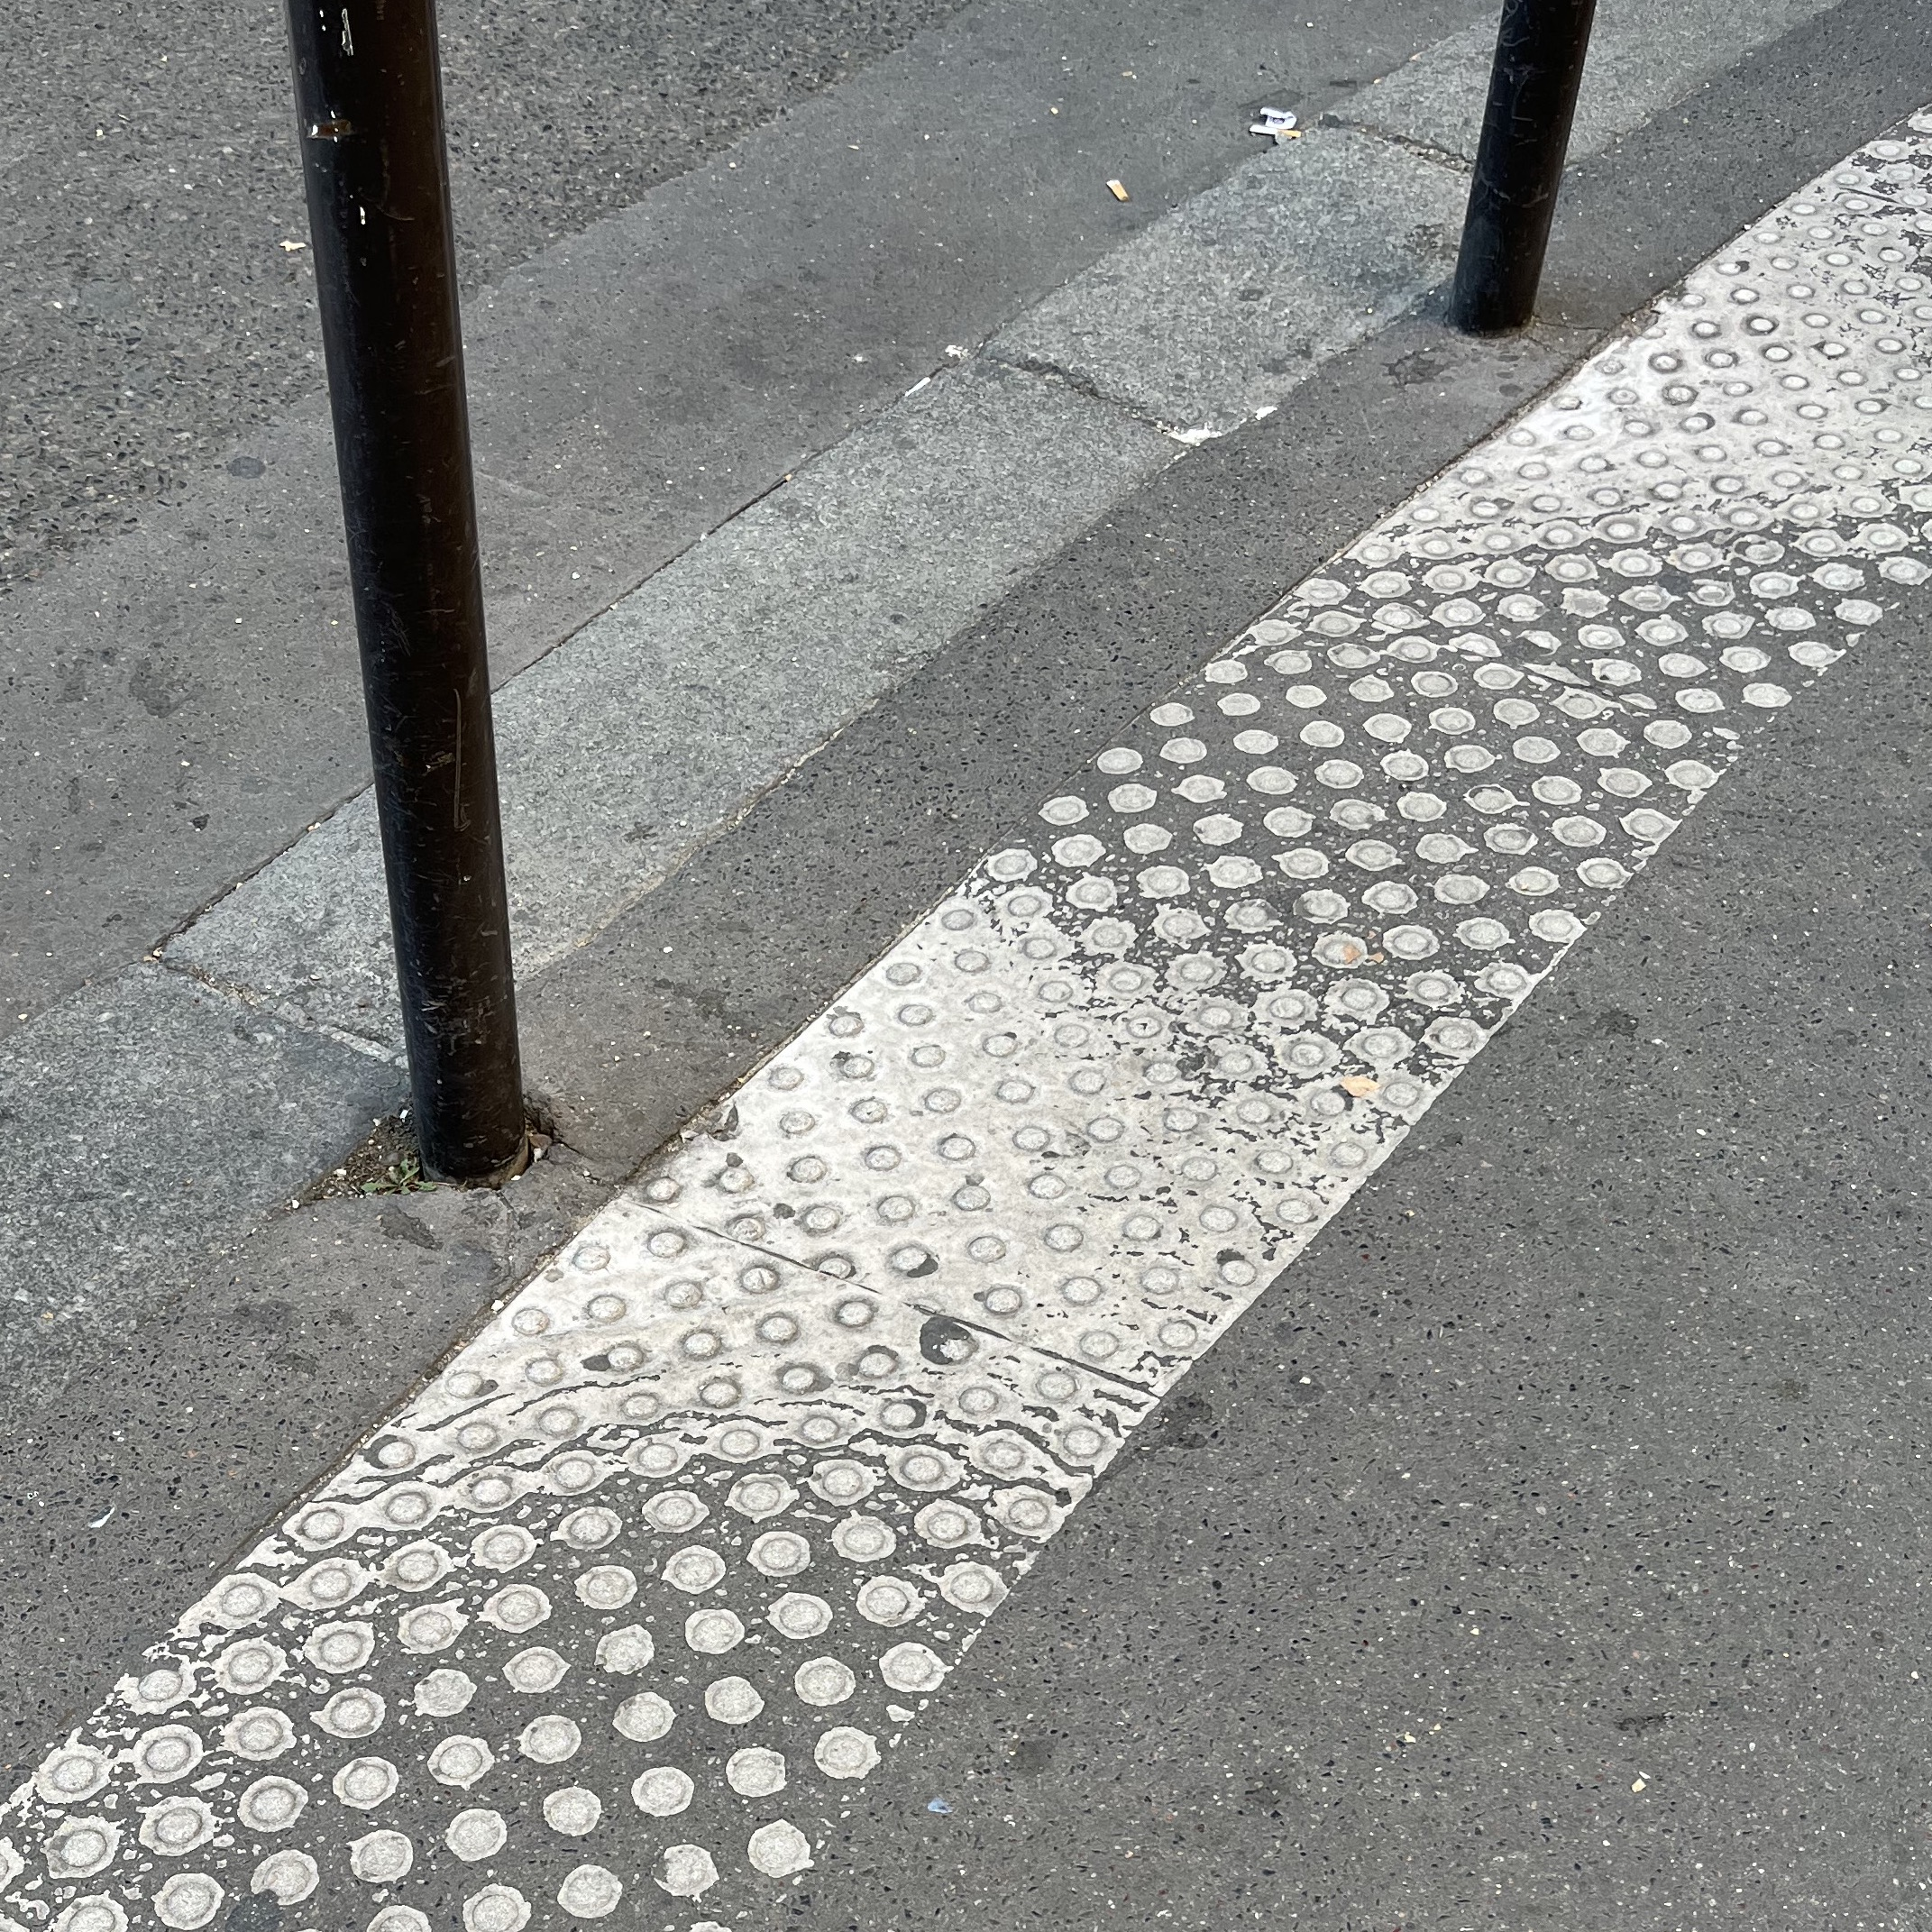
\includegraphics{images/modelisation/mod_bev.jpeg}} & Une \gls{bev} permet de détecter au pied ou à la canne la présence d'un passage piéton. On remarque sur l'image ci-contre qu'elle est abîmée, ce qui peut altérer sa détectabilité.\tabularnewline
        \resizebox{2cm}{!}{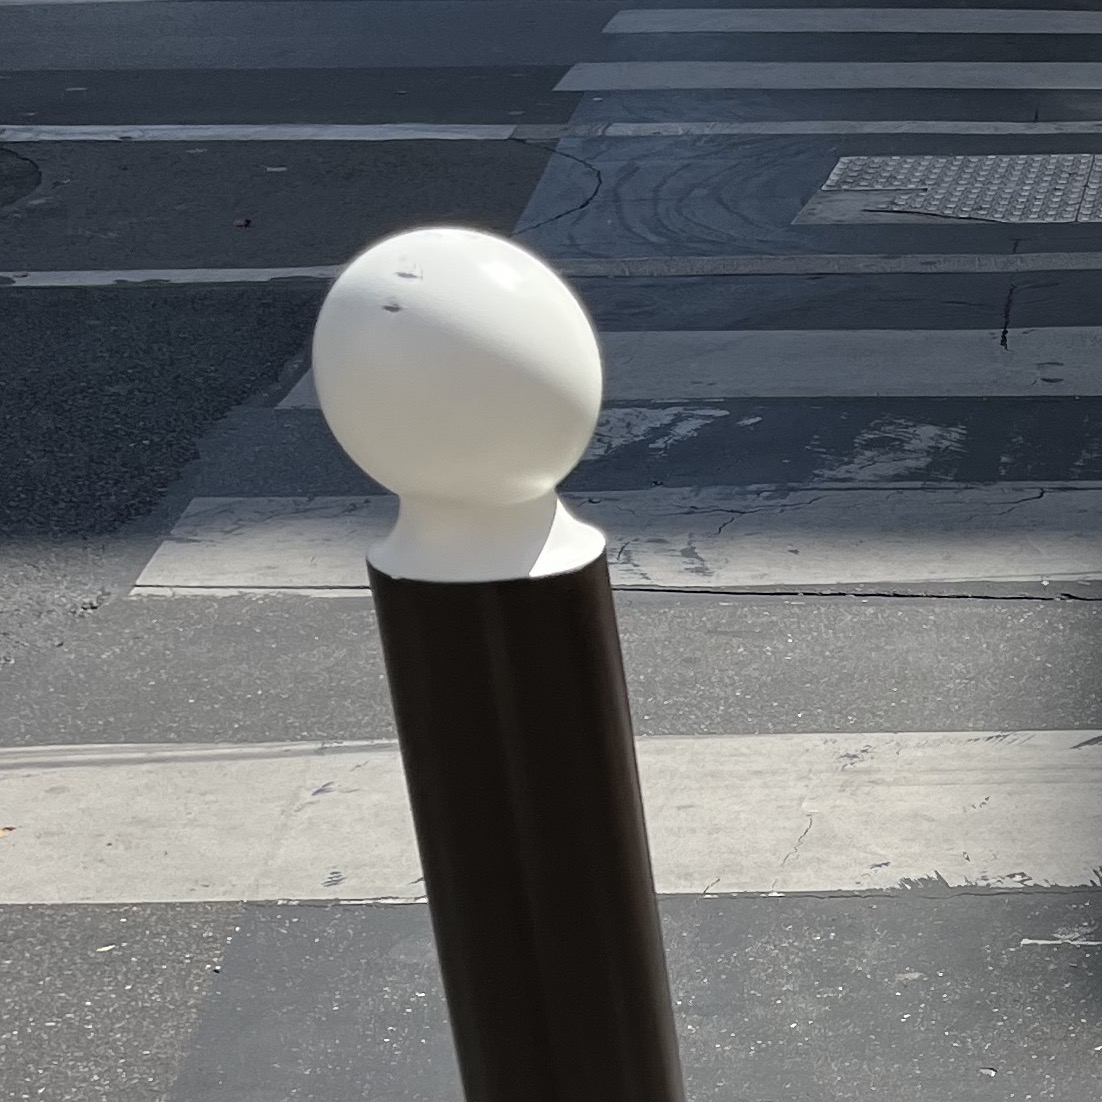
\includegraphics{images/modelisation/mod_poteau.jpeg}} & Les pôteaux parfois présents aux abords des passages piétons permettent à l'inster des \gls{bev} de signaler leur présence. Leur sommet est contrasté avec le corps pour permettre à une personne malvoyante de les distinguer.\tabularnewline
        \resizebox{2cm}{!}{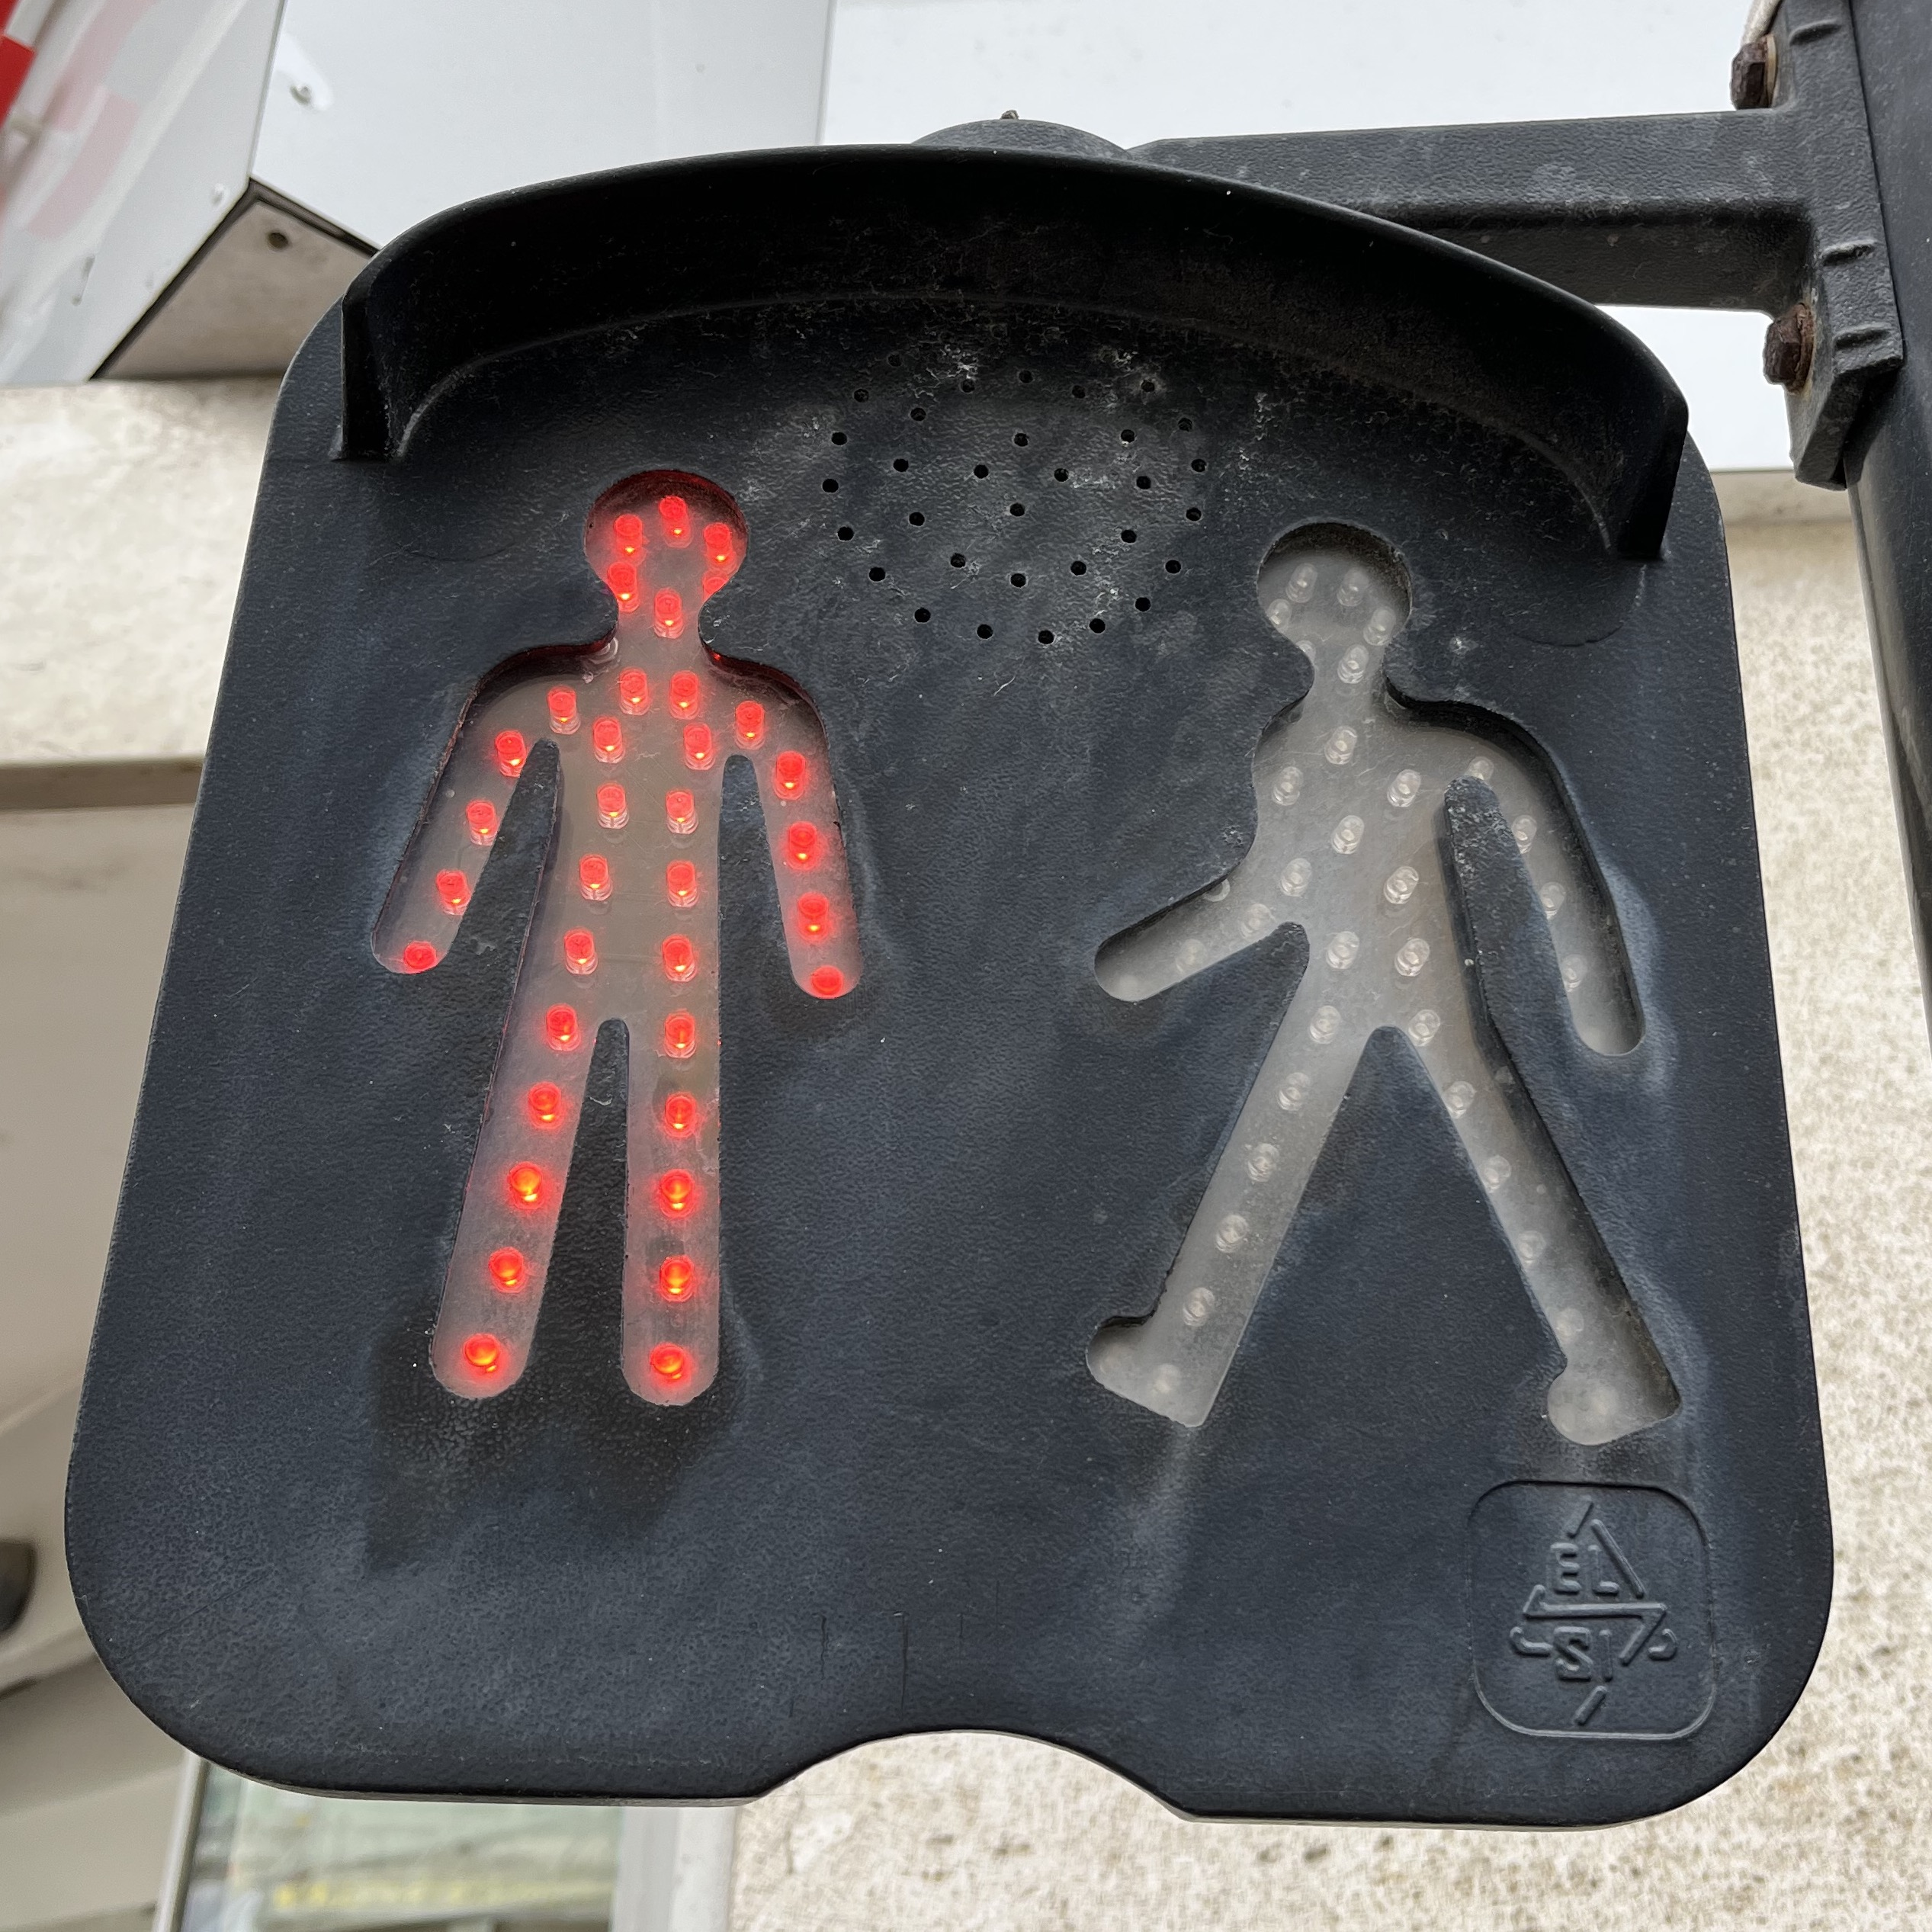
\includegraphics{images/modelisation/mod_feu_pieton.jpeg}} & Les feux de signalisation piéton peuvent être équipés d'une balise sonore. Le message joué par celle-ci varie, mais peut indiquer le nom de la rue traversée lorsque le feu est rouge. Un son de cloche est émis lorsque le feu est vert.\tabularnewline
    \end{tabular}
    \end{center}
    \caption{Équipements d'accessibilité au sein du carrefour.}
    \label{tab:modelisation_objets}
\end{table}

Au-delà des équipements d'accessibilité, le cycle des feux est également utile aux \glspl{pcdv} pour analyser la circulation et traverser en sécurité\comment{Citer une source, p-ê le manuel d'intervention ?}. Le cycle des feux correspond aux états successifs de chaque feu et permet de savoir quelles voies sont actuellement passantes. Il existe des modèles permettant la représentation de cette donnée, notamment au sein des outils de simulation de traffic routier\comment{Citer SUMO}. Cependant, il n'existe actuellement aucun territoire la rendant accessible au sein d'une source de données ouverte.

\section{La modélisation d’un carrefour au sein d’OpenStreetMap}

\label{sec:modelisation_osm}

% La délimitation des carrefours n'existe pas dans OSM.
% Celle des branches non-plus.

\gls{osm} est une base de données géographique libre sous licence ODbL. Une de ses spécificités concerne son ouverture aux contributions après inscription, la carte étant intégralement réalisée par les utilisateurs. Nous verrons dans cette partie que, si elle n'est pas particulièrement spécialisée pour la modélisation des carrefours, ses capacités de représentation et la couverture spatiale et sémantique actuelle de certaines données la rendent intéressante pour notre cas d'utilisation.

\subsection{Une forte capacité de représentation}

Plus qu'une base de données géographique, \gls{osm} est une base de données topologique\comment{Ajouter une citation}, pouvant être représentée sous la forme d'un graphe non-connexe. 3 types d'objets peuvent être manipulés pour cartographier une entité : les points (node), les lignes (way), et les relations, chacun pouvant contenir une sémantique sous la forme de clés et de valeurs associées (voir Figure \ref{fig:mod_ex_donnee_osm})

% Illustration qui représente une ligne de bus, composée de ways aggrégées au sein d'une relation.
\begin{figure}
    \centering
    
\includegraphics{images/placeholder.jpg}
    \caption{Les différents objets d'\gls{osm} peuvent chacun contenir des attributs.}
    \label{fig:mod_ex_donnee_osm}
\end{figure}

% L'accessibilité piétonne dans OSM

OpenStreetMap est très souple concernant la représentation de l'accessibilité piétonne, et permet de cartographier finement de nombreux aménagements. Il est ainsi possible de représenter un graphe piéton contenant sous forme linéaire les trottoirs et les passages piétons. Au-delà de la géométrie, la sémantique associée permet de compléter les informations liées à l'accessibilité. Sur un passage piéton, cela peut permettre d'indiquer la présence de \glspl{bev} (\osmkey{tactile\_paving}), d'un feu piéton (\osmvalue{traffic\_signals} pouvant être associée à plusieurs clés), et de préciser si ce dernier est sonorisé (\osmkey{traffic\_signals:sound}). On peut également faire figurer la bordure du trottoir (\osmkey{kerb}) et son élévation par rapport à la chaussée. Un exemple de cartographie de chemins piétons est illustré en Figure \ref{fig:modelisation_anatomie_carrefour_osm}.

\begin{figure}
    \centering
    \resizebox{15cm}{!}{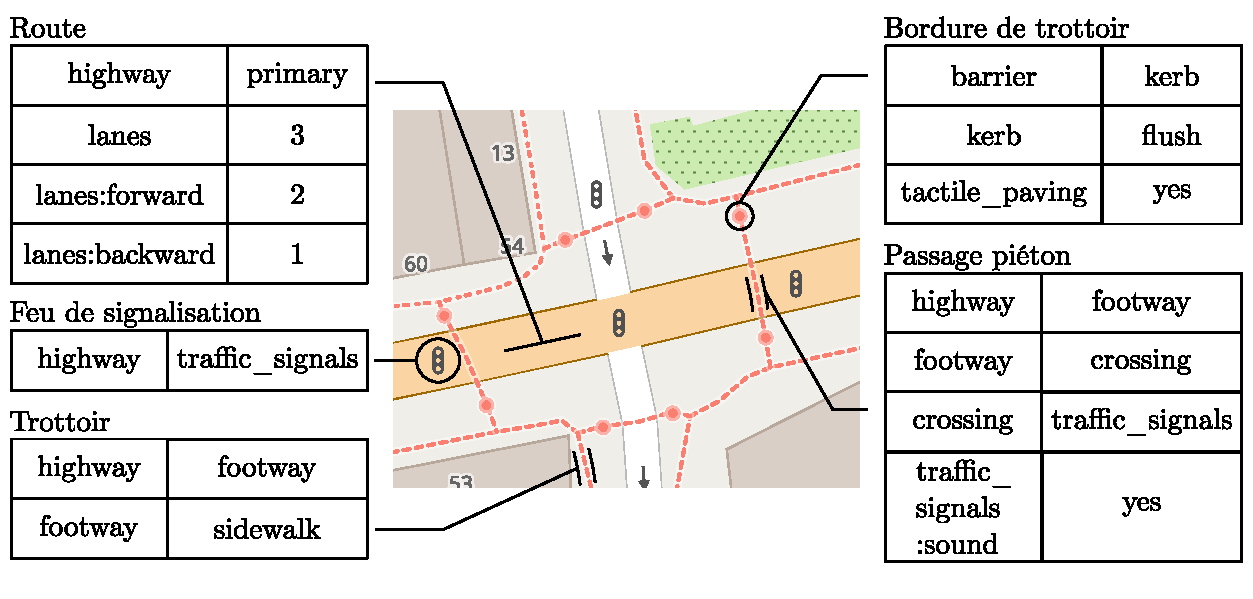
\includegraphics{images/modelisation/mod_anatomie_carrefour_osm.pdf}}
    \caption[Anatomie d'un carrefour dans OSM.]{Exemple de carrefour et des attributs associés dans OpenStreetMap. Outre le graphe piéton, des indications sur l'équipement d'accessibilité ou la largeur des voies (lanes) sont également présentes. Source : Contributeurs OpenStreetMap.}
    \label{fig:modelisation_anatomie_carrefour_osm}
\end{figure}

Au-delà de l'accessibilité de la voirie, la sémantique permet également de préciser l'accessibilité d'autres équipements. Cela vaut pour les bâtiments et commerces pour lesquels il est possible d'évaluer l'accessibilité d'une entrée (\osmkey{entrance}) en fauteuil roulant (\osmkey{wheelchair}) ainsi que la largeur de passage, mais également les aménagements tels que les arrêts de bus (\osmkey{highway}=\osmvalue{bus\_stop}) qui peuvent être abrités (\osmkey{shelter}) ou disposer d'un banc (\osmkey{bench}). Une illustration d'un cheminement comprenant des aménagements de ce type est proposé en Figure \ref{fig:mod_ex_accessibilite_eqp_osm}.

% Illustration d'une bordure de trottoir sur laquelle se trouve un arrêt de bus. Aux abords, un bâtiment dont la porte est modélisée. La sémantique est détaillée pour chaque objet.
\begin{figure}
    \centering
    
\includegraphics{images/placeholder.jpg}
    \caption{L'accessibilité de nombreux équipements peut être modélisée sur \gls{osm}.}
    \label{fig:mod_ex_accessibilite_eqp_osm}
\end{figure}

\newpar{}

% L'évolution de la sémantique sur OSM

Les clés et valeurs que nous évoquons se reposent sur la documentation établie par la communauté au sein du wiki d'\gls{osm}\footnote{https://wiki.openstreetmap.org/}. Si certaines clés et valeurs se sont imposées par l'usage (dit "de fait"\footnote{https://wiki.openstreetmap.org/wiki/Category:Key\_descriptions\_with\_status\_\%22de\_facto\%22}), la pratique usuelle pour faire évoluer la sémantique consiste à soumettre au vote de la communauté via le wiki une proposition de clés et valeurs supplémentaires pour représenter une nouvelle entité ou modifier un standard actuellement en vigueur. Nous pouvons illustrer cette pratique avec une donnée utile pour un piéton déficient visuel: le cycle des feux (evoqué en partie \ref{sec:mod_repere_carrefour}). S'il n'est pas possible avec la sémantique actuelle de représenter le cycle des feux sur \gls{osm}, un utilisateur propose en 2017 d'introduire une relation \osmkey{type}=\osmvalue{timing} \footnote{https://wiki.openstreetmap.org/wiki/Proposal:Traffic\_Signal\_Timings} pour modéliser cette information. Elle n'est pas, à l'heure actuelle, validée par la communauté car potentiellement inapplicables sur plusieurs territoires.

\newpar{}

% Ce que ne permet pas OpenStreetMap

La représentation des carrefours sur OpenStreetMap est en partie possible, mais ne correspond pas entièrement à notre besoin. Il existe la clé \osmkey{junction}, qui permet de pointer un carrefour voire de le délimiter (Figure \ref{fig:modelisation_carrefours_osm_paris}). Elle permet, au-delà de la valeur \osmvalue{yes} qui signifie que l'objet concerné est un carrefour, d'indiquer certains types de carrefour, en particulier les ronds-points avec la valeur \osmvalue{roundabout}\footnote{https://wiki.openstreetmap.org/wiki/Key:junction}. Cependant, la sémantique actuelle ne permet pas de modéliser les branches associées au carrefour. Par ailleurs, la plupart des carrefours ne sont pas représentés de cette manière.

\begin{figure}
    \centering
    \resizebox{15cm}{!}{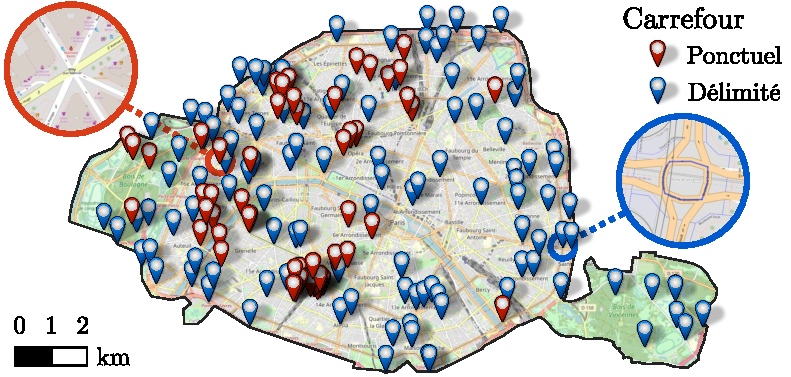
\includegraphics{images/modelisation/mod_carrefours_osm_paris.pdf}}
    \caption[Les carrefours OSM à Paris.]{À Paris, bien qu'il y ait beaucoup d'objets portant la clé \osmkey{junction}, la majorité des carrefours ne sont pas représentés sous cette forme. Source : Contributeurs OpenStreetMap.}
    \label{fig:modelisation_carrefours_osm_paris}
\end{figure}

\subsection{Des variations dans les modélisations}

\label{sec:modelisation_variation_pieton_osm}

% Variation dans la modélisation des trottoirs
% Variation dans la modélisation d'un passage piéton
% Etc.

Une particularité d'\gls{osm} est qu'il est possible de représenter les objets de plusieurs manières différentes. 

\todo{}

\section{Un modèle de carrefour}

Pour utiliser la donnée \gls{osm} dans un contexte spécifique, il est préconisé de la manipuler à l'aide d'un modèle de donnée spécialisé intermédiaire \cite{Touya2014}. Nous proposons dans un premier temps une modélisation objet générique de la donnée \gls{osm}, que nous appliquons dans un second temps à la modélisation du carrefour. Enfin, nous présentons les méthodes permettant d'instancier ce modèle depuis OpenStreetMap.

\subsection{OSM-Objet : une modélisation objet de la donnée OpenStreetMap}

\begin{figure}
\centering
\begin{plantuml}

    @startuml
    object Node {
        int id
        float x
        float y
    }

    object AbstractNode

    object NodeDecorator

    object Crosswalk
    object TrafficLight

    Node -r-|> AbstractNode
    NodeDecorator -u-|> AbstractNode
    AbstractNode "1" -* "1" NodeDecorator
    Crosswalk -u-|> NodeDecorator
    TrafficLight -u-|> NodeDecorator
    @enduml
    
\end{plantuml}
\caption[Modèle OSM-Objet.]{Modèle OSM-Objet. Les classes Crosswalk et TrafficLight sont présentes pour illustrer l'utilisation.}
\label{fig:modelisation_osm_objet}
\end{figure}

Comme présenté dans la partie \ref{sec:modelisation_osm}, les objets représentés au sein d'\gls{osm} sont définis par un ensemble de clés et de valeurs. Ainsi, pour manipuler chaque objet, il est nécessaire de déterminer l'ensemble des clés et valeurs qui vont le définir. En ce sens, il est plus commode de manipuler un modèle intermédiaire pour lequel cet ensemble est prédéfini. Cette problématique a déjà été abordée au sein des ontologies réalisées autour d'\gls{osm}\cite{Codescu2011,Hombiat2017} ou des travaux qui s'appuient sur ces données \cite{Touya2014}. Cependant, une particularité des capacités sémantique d'OpenStreetMap est qu'il est possible que la somme des clés et des valeurs d'une entité corresponde à plusieurs objets dans la vie réelle. Un exemple typique concerne les passages piétons représentés par un nœud et dont la sémantique contient souvent à la fois celle associée au passage piéton, ainsi que celle associée au feu de circulation. Pour gérer cette particularité, nous proposons un modèle de données orienté objet appelé OSM-Objet.

\newpar{}

OSM-Objet se repose sur le patron de conception du décorateur \cite{Gamma1994a}. Le décorateur permet d'ajouter dynamiquement des fonctionnalités à un objet sans passer par une sous-classe, et en conservant la même interface pour le manipuler. Dans notre cas, comme l'illustre la figure \ref{fig:modelisation_osm_objet}, nous pouvons manipuler un nœud, qui peut être simultanément un passage piéton et un feu de signalisation.

\subsection{Application à la modélisation du carrefour}

\begin{figure}
    \centering
    \begin{plantuml}
        @startuml

        enum Direction {
            IN
            OUT
        }

        object Lane {
            int id
        }
        object Bus
        object Road

        object Way {
            int id
            string name
        }

        object Node {
            int id
            float x
            float y
        }
        object AbstractNode
        object NodeDecorator
        object TrafficLight
        object PedestrianTrafficLight
        object Crosswalk

        object Branch {
            int id
        }

        object Intersection

        object PedestrianNode {
            int id
        }
        object Sidewalk
        object Island
        object Crossing

        'Relations

        'Decorator part
        Node -r-|> AbstractNode
        NodeDecorator -l-|> AbstractNode
        AbstractNode "1" -r-* "1" NodeDecorator
        TrafficLight -u-|> NodeDecorator
        PedestrianTrafficLight -u-|> NodeDecorator
        Crosswalk -u-|> NodeDecorator

        'Way part
        Way "*" o-r- "2" Node

        'Lanes part
        Way "1" *-u- "*" Lane
        Lane <|-r- Bus
        Lane <|-r- Road
        Lane o-l- Direction

        'Branch part
        Branch "1" o-r- "*" Way
        Intersection "1" *-r- "*" Branch
        Branch "1" *-d- "1" Crossing

        'Pedestrian node part
        Way "*" o-d- "0..2" PedestrianNode
        Sidewalk -r-|> PedestrianNode
        Island -l-|> PedestrianNode
        PedestrianNode "2" -d-o "*" Crosswalk

        'Crossing part
        Crossing o-r- Crosswalk

        'Placement commands
        PedestrianTrafficLight -d[hidden]- TrafficLight
        Crosswalk -u[hidden]- PedestrianTrafficLight

        @enduml 
    \end{plantuml}
    \caption[Modèle CrModel.]{Modèle CrModel architecturé autour d'OSM-Objet.}
    \label{fig:modelisation_crmodel}
\end{figure}

Pour modéliser le carrefour, nous proposons CrModel, le modèle de données en figure \ref{fig:modelisation_crmodel}. Il représente un graphe du carrefour, dont la classe Node figure les nœuds et la classe Way figure les tronçons. Nous avons architecturé les nœuds autour d'OSM-Objet. Chaque branche (Branch) est identifiée par un numéro et contient tous les tronçons qui en font partie. Une  branche peut également contenir une traversée (Crossing). Nous avons également introduit certains comportements spécifiques:

\begin{itemize}
    \item Les différentes voies d'une route sont identifiées par des attributs sur \gls{osm}. Nous avons donc ajouté la classe Lane pour représenter cette information dans un paradigme objet.
    \item Les trottoirs (Sidewalk) et les îlots (Island) sont également des classes indépendantes et non de la sémantique sur les tronçons. Chaque tronçon peut contenir deux PedestrianNode, permettant d'indiquer quel trottoir ou îlot est à sa droite ou à sa gauche.
    \item Nous voulons pouvoir indiquer pour chaque branche si et comment elle se traverse. Pour cela, nous avons introduit la classe Crossing qui consiste en une séquence de passages piétons entre deux trottoirs. Les passages piétons eux-même sont composés de deux PedestrianNode qui indiquent où se situe le passage piéton (entre un trottoir et îlot par exemple).
\end{itemize}

\newpar{}

La partie suivante détaille la manière d'instancier ce modèle depuis OpenStreetMap.

\section{Instancier le modèle depuis OpenStreetMap}

Instancier CrModel repose sur trois grandes étapes:
\begin{itemize}
    \item Segmenter le graphe d'OpenStreetMap pour délimiter le carrefour et ses branches
    \item Augmenter la donnée en calculant les trottoirs et les traversées
    \item Utiliser les résultats précédents pour construire CrModel
\end{itemize}

Ces dernières seront détaillées dans les parties suivantes.

\newpar{}

Comme évoqué précédemment, sur \gls{osm}, la donnée piétonne bien qu'évoluant favorablement est aujourd'hui parcellaire, notamment en ce qui concerne un réseau piéton indépendant du réseau routier. Ce dernier contenant cependant une partie des informations liées à la piétonnisation dans la sémantique de ses arêtes (trottoirs) et de ses nœuds (passages piéton), les travaux présentés dans cette partie se reposeront exclusivement sur le réseau routier.

\subsection{Segmenter un carrefour dans le graphe d'OpenStreetMap}

\subsubsection{Définition de la segmentation}

Cette sous-partie est issue de travaux réalisés en collaboration avec Jean-Marie Favreau. Elle se repose sur les définitions proposées en partie \ref{sec:modelisation_definitions}.

\newpar{}

\begin{figure}
    \centering
    \begin{subfigure}[t]{.49\linewidth}
        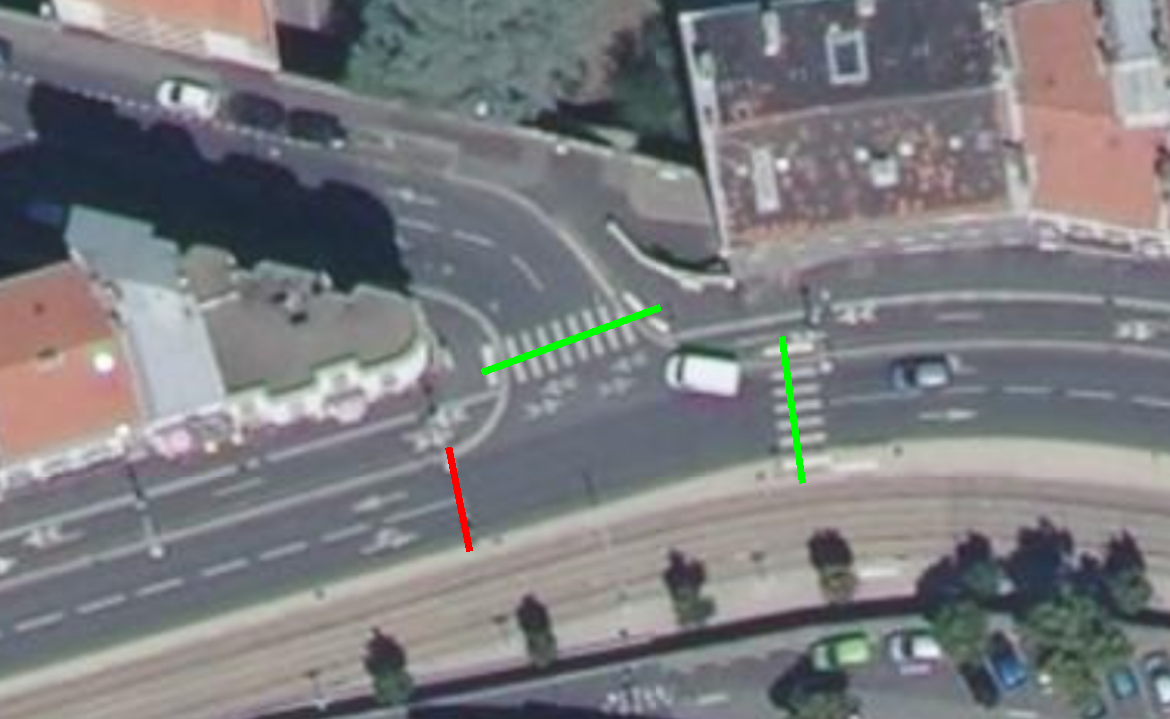
\includegraphics[width=\textwidth]{images/modelisation/segmentation/orthophoto-1.pdf}
        \caption{Un carrefour dont les bordures sont définies par deux passages piétons (lignes vertes) et un feu de signalisation (ligne rouge).\label{fig:modelisation_limite_carrefourA}}
    \end{subfigure}
    \begin{subfigure}[t]{.49\linewidth}
        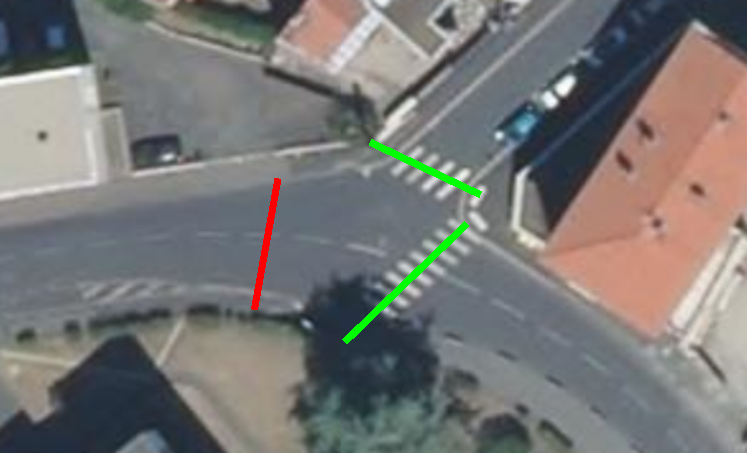
\includegraphics[width=\textwidth]{images/modelisation/segmentation/orthophoto-2.pdf}
        \caption{Un carrefour dont les bordures sont définies par deux passages piétons (lignes vertes) et une branche sans marquage (ligne rouge). \label{fig:modelisation_limite_carrefourB}}
    \end{subfigure}
    \caption{Les bordures des carrefours sont situées au niveau des infrastructures, si elles existent. Fond de plan: Géoportail © IGN. Source: \cite{Favreau2022}.}
    \label{fig:modelisation_limite_carrefour}
\end{figure}

Du point de vue d'un piéton, la bordure entre le cœur de carrefour et les branches (voir définition \ref{def:modelisation_couverture_routiere_complète}) sera généralement située au niveau des passages piétons pour chaque branche du carrefour. Si une branche n'a pas de passage piéton, cette séparation sera située là où les véhicules s'arrêtent (feu de circulation, panneau stop, etc.) comme illustré à la figure \ref{fig:modelisation_limite_carrefourA}. En cas d'absence de toute signalisation, la limite sera placée aussi près que possible pour éviter d'étendre sa zone dans la branche adjacente, comme illustré à la figure \ref{fig:modelisation_limite_carrefourB}.

\newpar{}

Comme évoqué en partie \ref{sec:modelisation_variation_pieton_osm} l'infrastructure piétonne est aujourd'hui encore rarement modélisée séparément de la route. Par conséquent, nous proposons dans la suite de cette partie de considérer uniquement la donnée contenue par les nœuds et arêtes du réseau routier. Nous supposons que les informations suivantes (reconstruites ou directement disponibles) sont accessibles sur le réseau routier:

\begin{itemize}
    \item La largeur de la route, directement accessible (\osmkey{width}) ou estimée en fonction du type de route (\osmkey{highway}) et du nombre de voies (\osmkey{lanes}),
    \item le type de route, si elle correspond à un carrefour (\osmkey{junction} ou \osmkey{highway} = \osmvalue{*\_link}),
    \item le nom de la route (\osmkey{name}),
    \item le type du nœud s'il décrit un élément de l'infrastructure (clé \osmkey{highway}): passage piéton (\osmvalue{crossing}), feu de circulation (\osmvalue{traffic\_signal}), panneau stop (\osmvalue{stop}) ou cédez-le-passage (\osmvalue{give\_way}).
\end{itemize}

\newpar{}

\begin{figure}
    \centering
    \resizebox{15cm}{!}{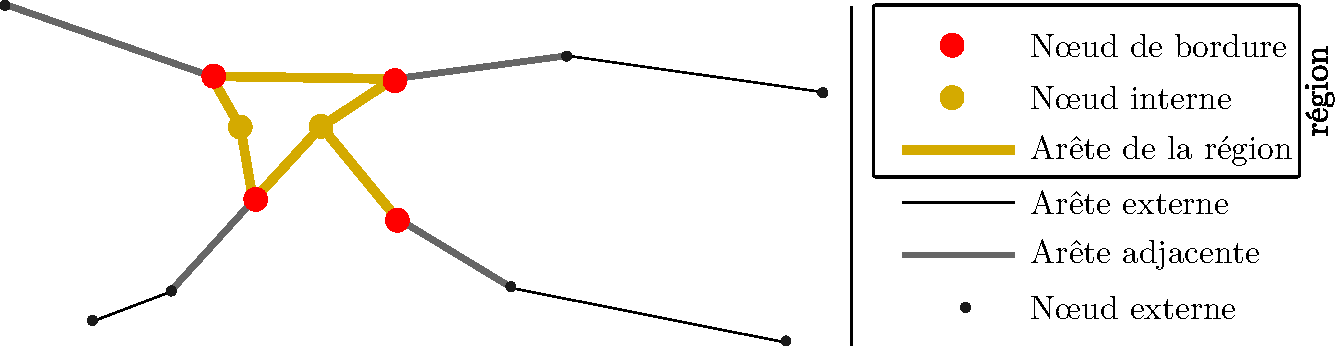
\includegraphics{images/modelisation/segmentation/region.pdf}}
    \caption{Exemple de région définie dans le graphe. Source: \cite{Favreau2022}.}
    \label{fig:modelisation_region_segmentation}
\end{figure}

On considère un graphe routier $G_r = (V_r,E_r)$ dont les nœuds et les arêtes contiennent des informations sémantiques sous la forme de clés-valeurs. Nous définission une segmentation du graphe routier en identifiant pour chaque région de la segmentation un ensemble non-vide de nœuds et un ensemble possiblement vide d'arêtes, avec la contrainte suivante : si une arête appartient à une région, ses deux nœuds lui appartiennent également.
Pour chaque région, nous identifions deux types de nœuds: les \textbf{nœuds internes} (uniquement connectés aux arêtes appartenant à la région), et les \textbf{nœuds de bordure} (connectés à au moins une arête appartenant à la région, et une arête n'appartenant pas à la région) (voir figure \ref{fig:modelisation_region_segmentation}).
Les \textbf{arêtes adjacentes} d'une région sont identifiées comme les arêtes qui n'appartiennent pas à la région, mais dont un une des extrêmités en fait partie.

\subsubsection{Carrefour élémentaire}

La première étape de la détection des carrefours que nous proposons consiste à évaluer pour chaque nœud la probabilité qu'il s'agisse d'un nœud interne ou d'un nœud de bordure d'un carrefour.
Cette première identification nous permet de caractériser:

\begin{itemize}
    \item Les passages piétons comme probables nœuds de bordure d'un carrefour
    \item Les nœuds représentant les entités de contrôle du traffic (feu de signalisation, panneaux stop et cédez-le-passage) comme possibles nœuds de bordure d'un carrefour
    \item Les nœuds avec une cardinalité supérieure à deux, et dont les arêtes adjacentes ont des noms de rue distincts, comme probablement nœuds internes d'un carrefour, et considérés comme nœuds graine dans les étapes suivantes de l'algorithme
\end{itemize}

\begin{figure}
    \centering
    \begin{subfigure}[t]{.49\linewidth}
        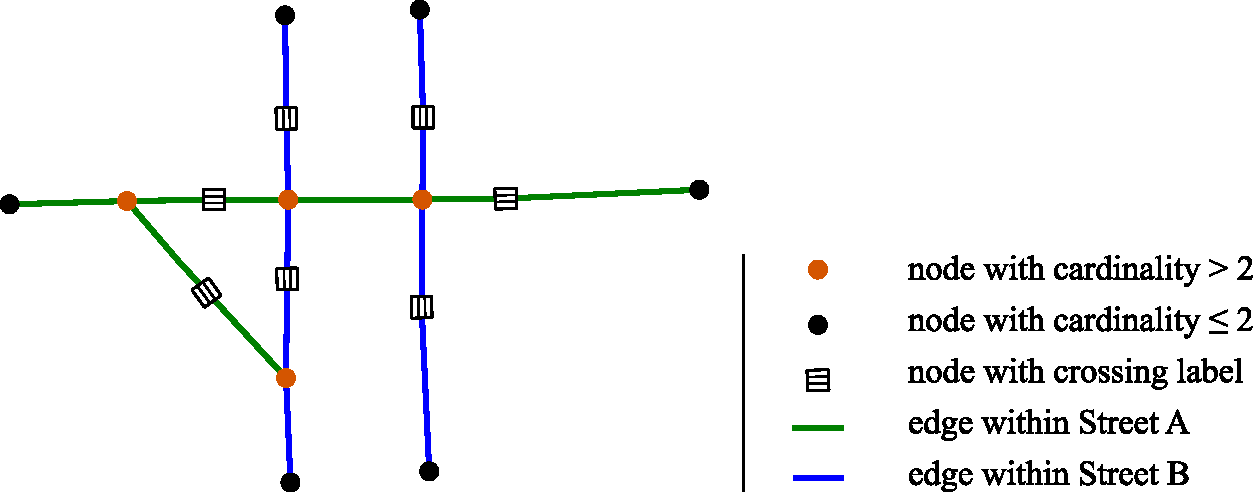
\includegraphics[width=\textwidth]{images/modelisation/segmentation/segmentation-step1.pdf}
        \caption{Un graphe labellisé tel qu'il peut être extrait d'\gls{osm}.\label{fig:modelisation_segmentation_step1}}
    \end{subfigure}
    \begin{subfigure}[t]{.49\linewidth}
        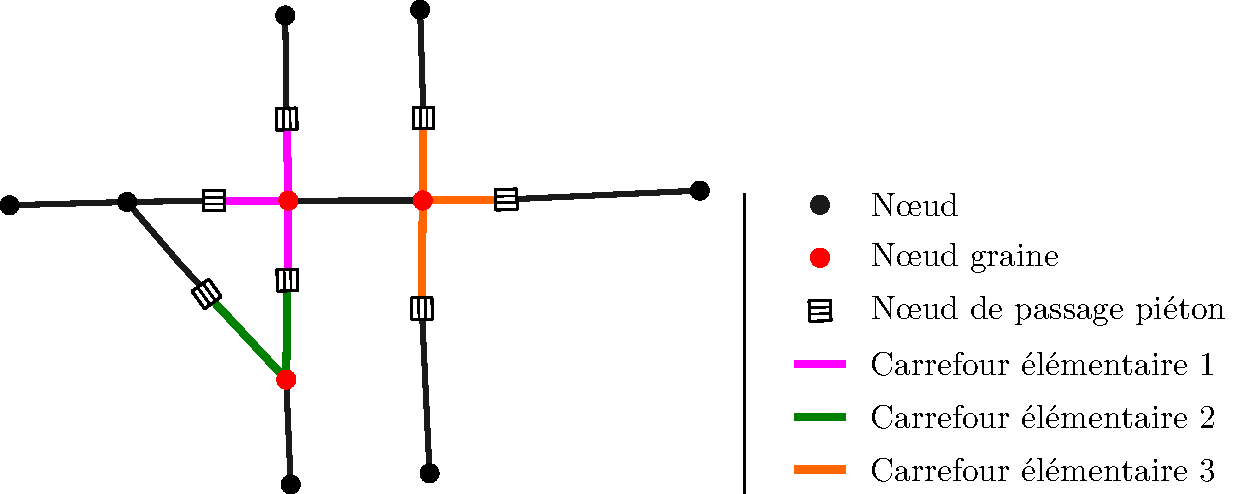
\includegraphics[width=\textwidth]{images/modelisation/segmentation/segmentation-step2.pdf}
        \caption{Carrefours élémentaires générés depuis le graphe de gauche. \label{fig:modelisation_segmentation_step2}}
    \end{subfigure}
    \caption{Résultat de la segmentation d'un carrefour élémentaire. Source: \cite{Favreau2022}.}
    \label{fig:modelisation_segmentation_step1&2}
\end{figure}

\newpar{}

De cette première identification (voir figure \ref{fig:modelisation_segmentation_step1}), nous détaillons dans la partie \ref{sec:implementation_segmentation} l'implémentation qui permet de construire les carrefours élémentaires, en utilisant la sémantique de la voie pour guider la décision d'étendre et consolider la segmentation de chaque nœud graine (voir figure \ref{fig:modelisation_segmentation_step2}).

\subsubsection{Approche multi-échelle}

\begin{figure}
    \centering
    \begin{subfigure}[t]{.49\linewidth}
        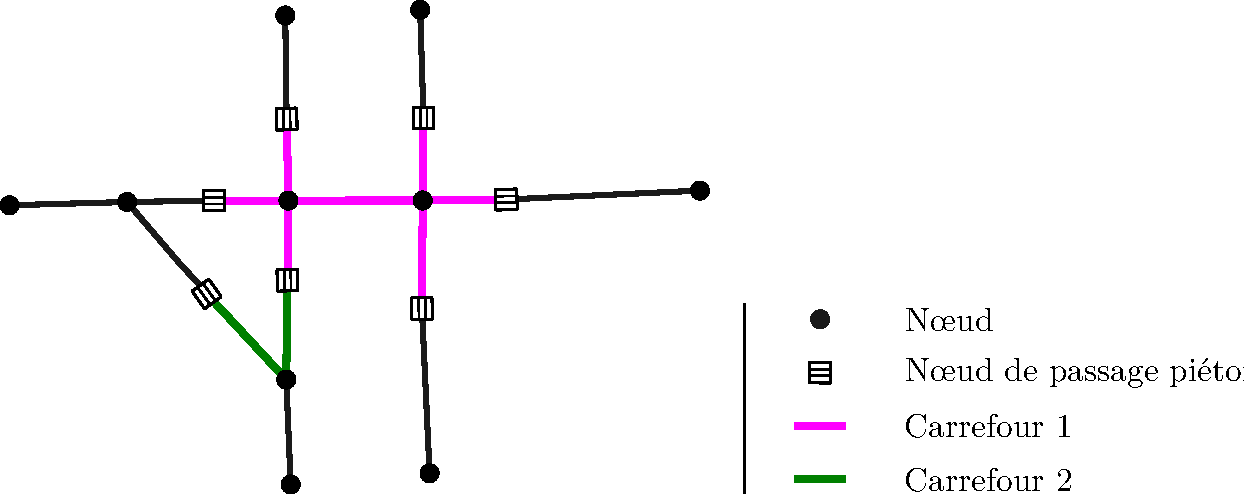
\includegraphics[width=\textwidth]{images/modelisation/segmentation/segmentation-step3.pdf}
        \caption{Résultat de la première étape d'assemblage des carrefours élémentaires de la figure \ref{fig:modelisation_segmentation_step2}.\label{fig:modelisation_segmentation_step3}}
    \end{subfigure}
    \begin{subfigure}[t]{.49\linewidth}
        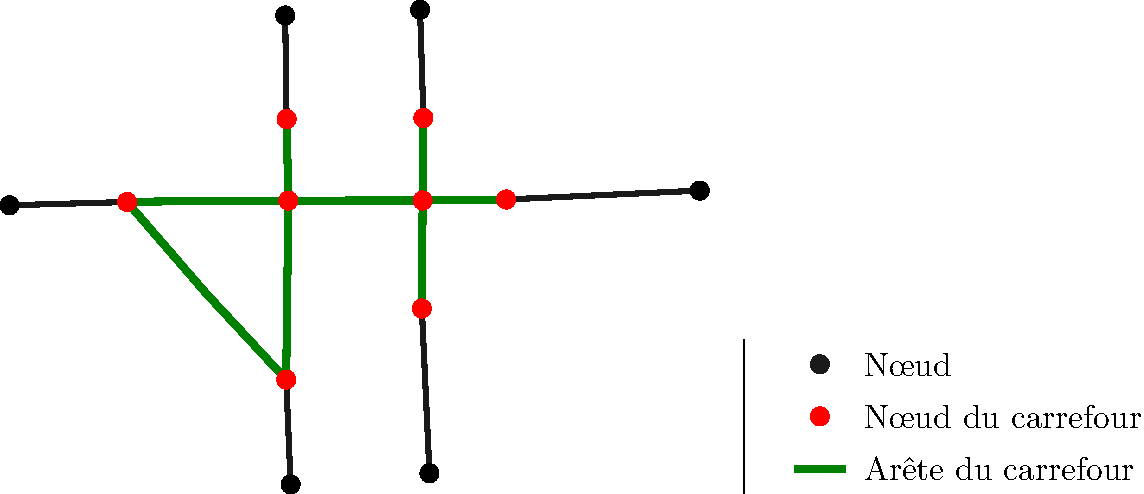
\includegraphics[width=\textwidth]{images/modelisation/segmentation/segmentation-step4.pdf}
        \caption{Résultat de la seconde étape d'assemblage des carrefours de gauche.\label{fig:modelisation_segmentation_step4}}
    \end{subfigure}
    \caption{Résultat de l'assemblage des carrefours élémentaires. Source: \cite{Favreau2022}.}
    \label{fig:modelisation_segmentation_step3&4}
\end{figure}

La segmentation de la partie précédente ne correspond pas réellement à l'intuition d'un piéton. En effet, elle produit plusieurs petites régions souvent proches les unes des autres. Cependant, nous pouvons identifier ces dernières comme des sous-parties d'un carrefour plus complexe. En utilisant la sémantique, la géométrie et la topologie des arêtes adjacentes à chaque carrefour, nous proposons un algorithme pour assembler les carrefours élémentaires en carrefours fonctionnels.

\newpar{}

La première étape d'assemblage consiste à identifier des couples de carrefours connectés par un chemin court, et qui ont des arêtes adjacentes orthogonales à ce chemin et portant le même nom de rue (voir figure \ref{fig:modelisation_segmentation_step3}). La seconde étape consiste ensuite à identifier les ensembles de carrefours connectés par un cycle court, et de les aggréger en carrefours fonctionnels. Cela nous permet de prendre en compte les carrefours complexes avec des voies de tourne-à-droite, ou des carrefours comportant plusieurs routes internes (voir figure \ref{fig:modelisation_segmentation_step4}). 

\newpar{}

Dans ces deux étapes d'assemblage, la notion de "court" est construite proportionnelement à la largeur de la voie, et en considérant la sémantique des arêtes appartenant au carrefour. Par exemple, si une arête est labellisée comme partie d'un carrefour, alors sa longueur est diminuee. Le chemin résultant est comparé à la largeur de la voie (voir \ref{sec:implementation_segmentation}).

\subsubsection{Segmentation des branches}

\begin{figure}
    \centering
    \resizebox{15cm}{!}{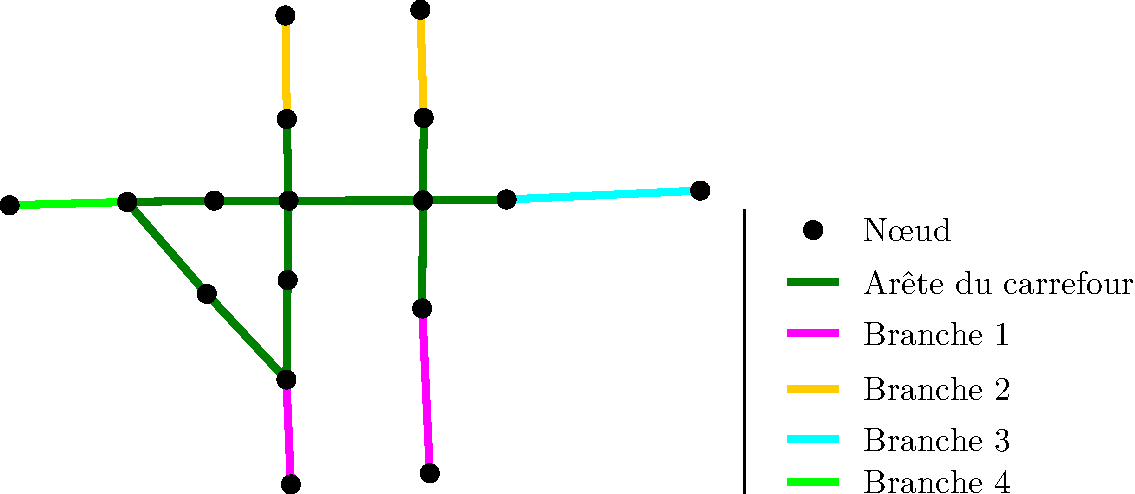
\includegraphics{images/modelisation/segmentation/segmentation-step5.pdf}}
    \caption{Segmentation des branches depuis le carrefour fonctionnel de la figure \ref{fig:modelisation_segmentation_step4} et utilisant les noms de rue donnés en figure {\ref{fig:modelisation_segmentation_step1}}. Source: \cite{Favreau2022}.}
    \label{fig:modelisation_segmentation_step5}
\end{figure}

Si la chaussée est complexe, il peut arriver que les branches d'un carrefour soit composées de plusieurs arêtes, par exemple en présence d'un séparateur de voies ou d'un îlot. La dernière étape de la segmentation consiste à regrouper les arêtes par branches en utilisant leurs informations géométriques et sémantiques (voir figure \ref{fig:modelisation_segmentation_step5}).

\subsection{Calcul des informations piétonnes}

\subsubsection{Aggrégation des trottoirs}

\begin{figure}
    \centering
    \resizebox{15cm}{!}{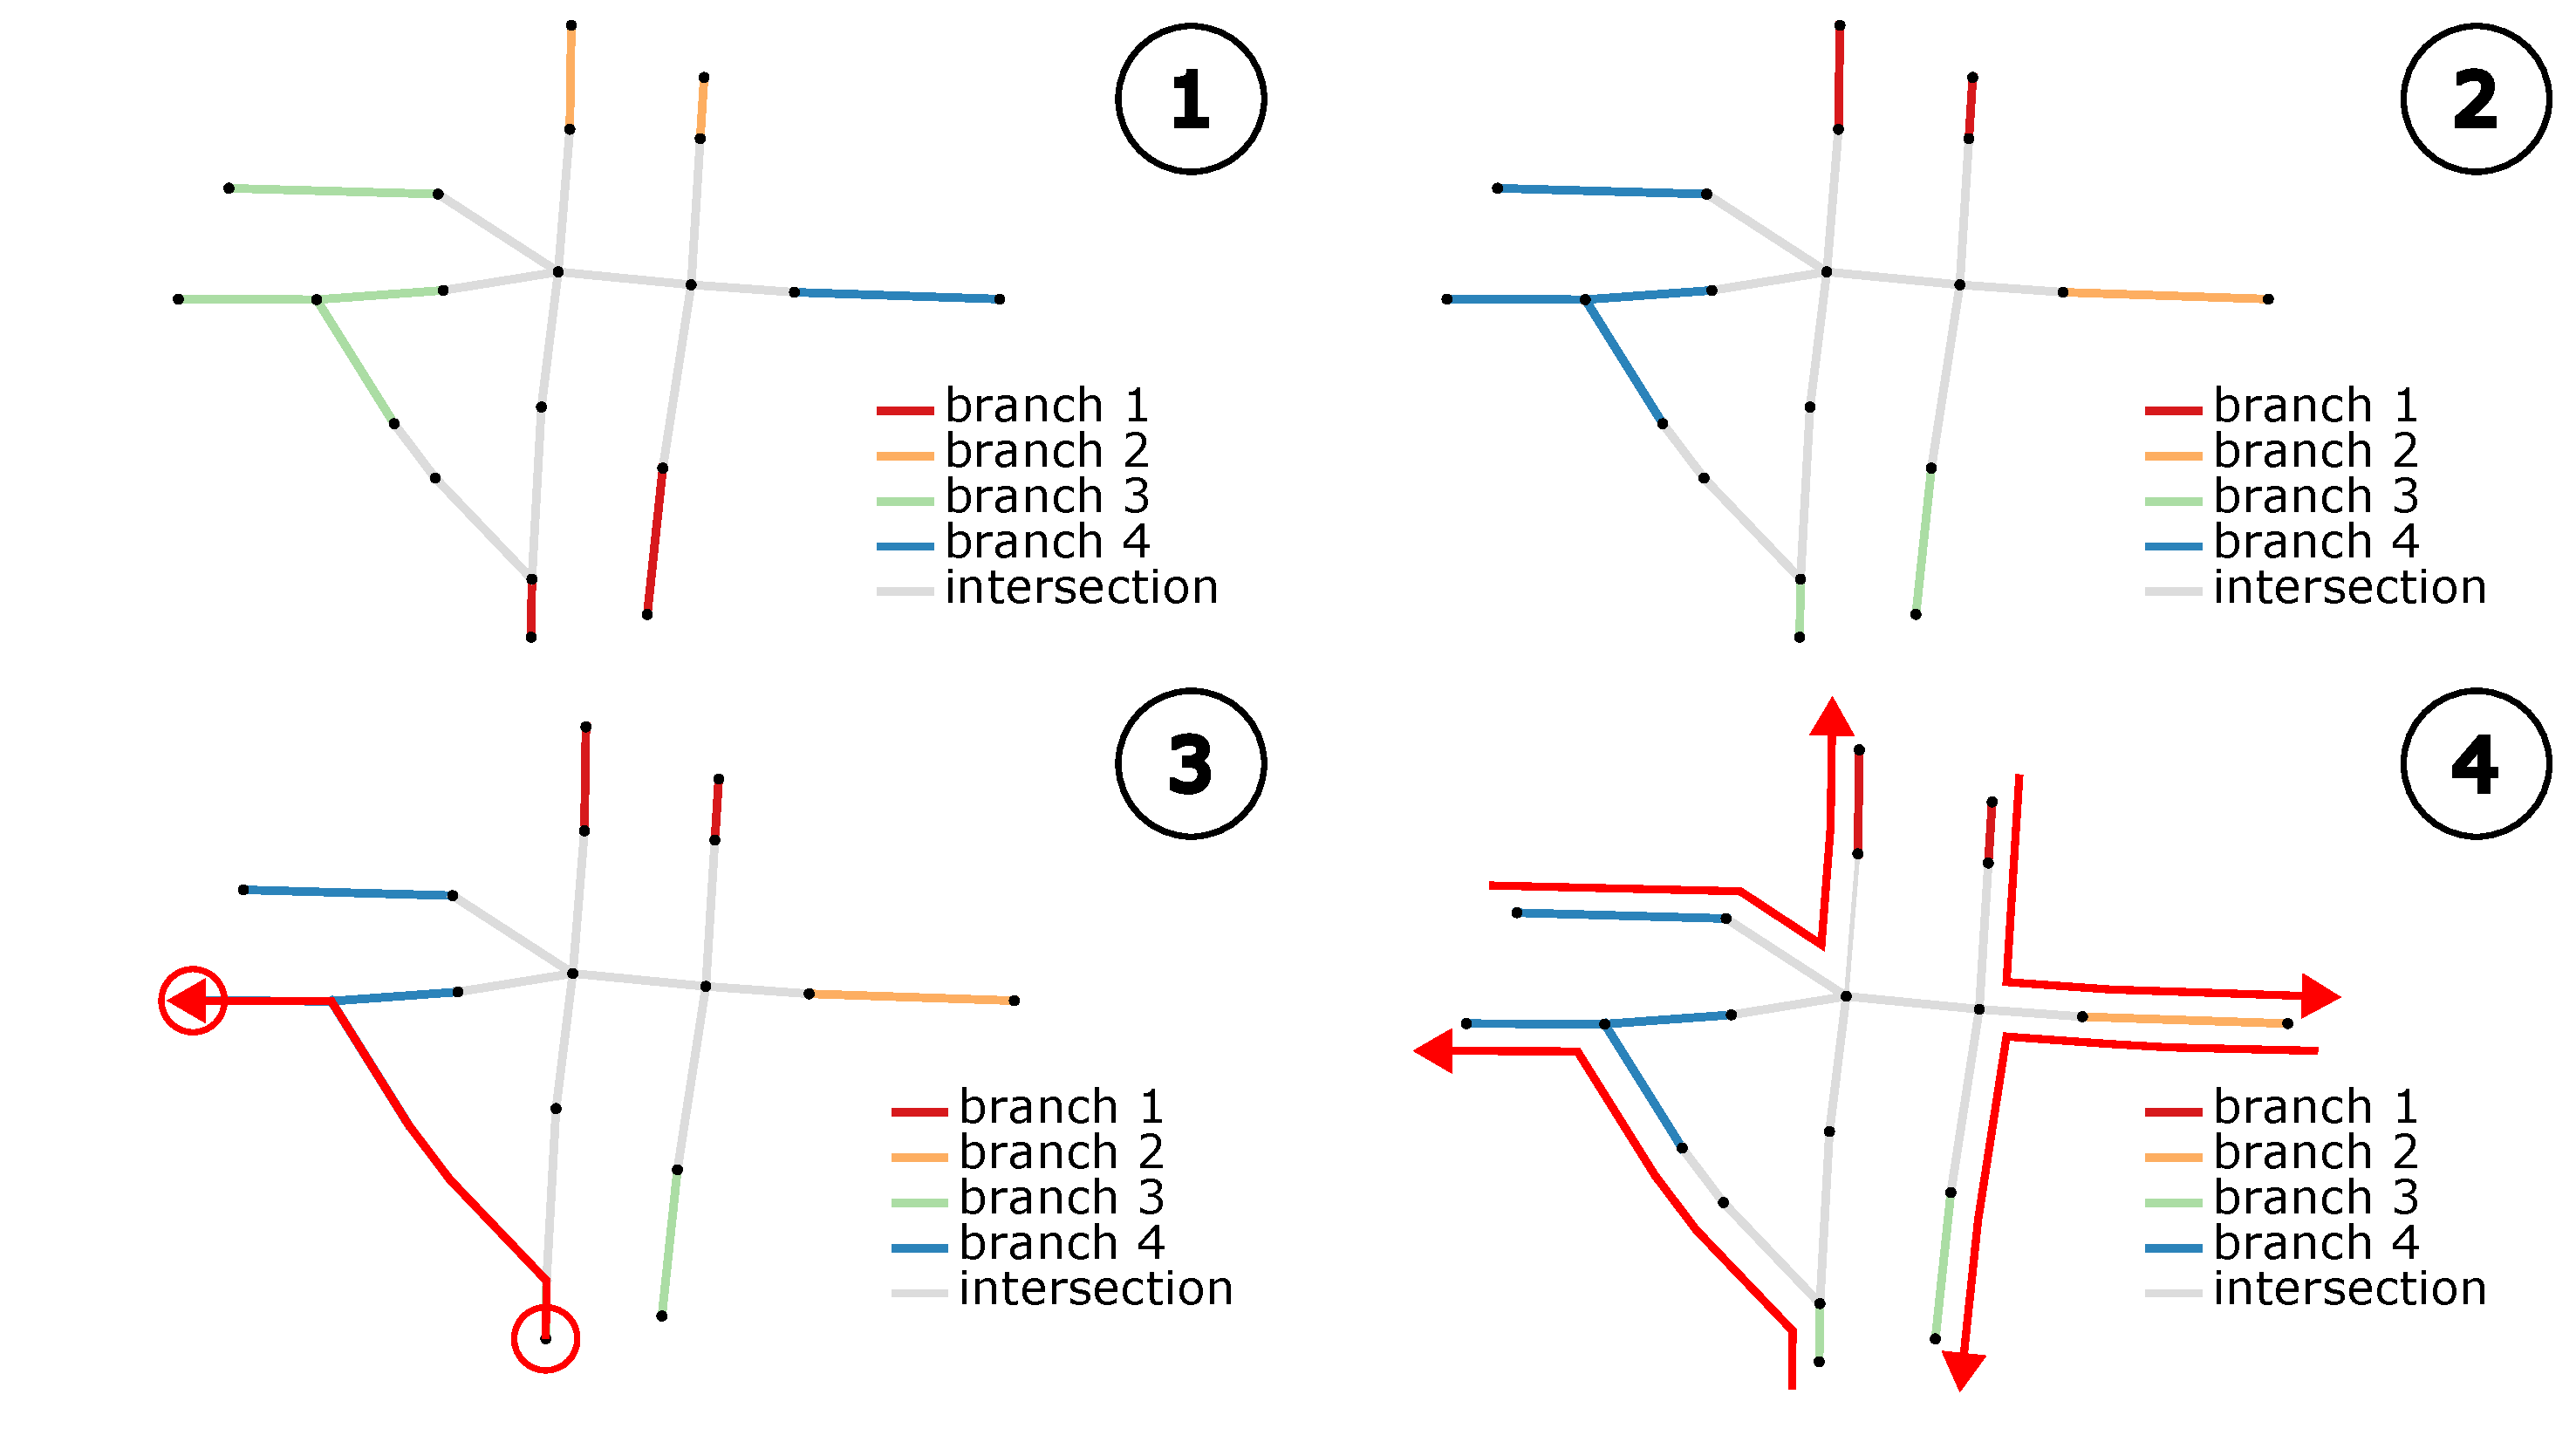
\includegraphics{images/modelisation/calcul_pieton/sidewalks.pdf}}
    \caption{Étapes de génération des trottoirs. Source: \cite{Kalsron2022}.}
    \label{fig:modelisation_calcul_pieton_trottoirs}
\end{figure}

Dans \gls{osm}, les trottoirs identifiés sous forme de sémantique sur le réseau routier ne sont pas aggrégés en une entité unique: chaque tronçon de route indique s'il présente ou non un trottoir à sa droite ou à sa gauche. Si l'on veut considérer une entité trottoir complète, il est nécessaire d'aggréger les tronçons correspondants et déterminer de quel côté le trottoir est situé.

La génération est réalisée de la manière suivante: d'abord, les branches issues de la segmentation (voir figure \ref{fig:modelisation_segmentation_step5}) ne sont pas ordonnées, donc nous les ordonnons dans le sens des aiguilles d'une montre (voir figure \ref{fig:modelisation_calcul_pieton_trottoirs}.2). Pour chaque branche du carrefour, une par une dans le sens des aiguilles d'une montre, on part du nœud situé à l'extrémité de l'arête la plus à droite et on parcours le graphe en tournant toujours à gauche jusqu'à atteindre une seconde extrêmité (voir figure \ref{fig:modelisation_calcul_pieton_trottoirs}.3). Le chemin traversé correspond alors à un trottoir (voir figure \ref{fig:modelisation_calcul_pieton_trottoirs}.4). Si l'arête est traversée dans sa direction, le trottoir est situé à sa gauche, sinon il est situé à sa droite. Si aucune sémantique n'indique l'absence de trottoir, on considère qu'il est présent. Nous avons fait ce choix car la majorité des villes ont des trottoirs, et la donnée \gls{osm} n'est pas encore suffisamment renseignée sur la sémantique associée.

\subsubsection{Génération des îlots}

\begin{figure}
    \centering
    \resizebox{15cm}{!}{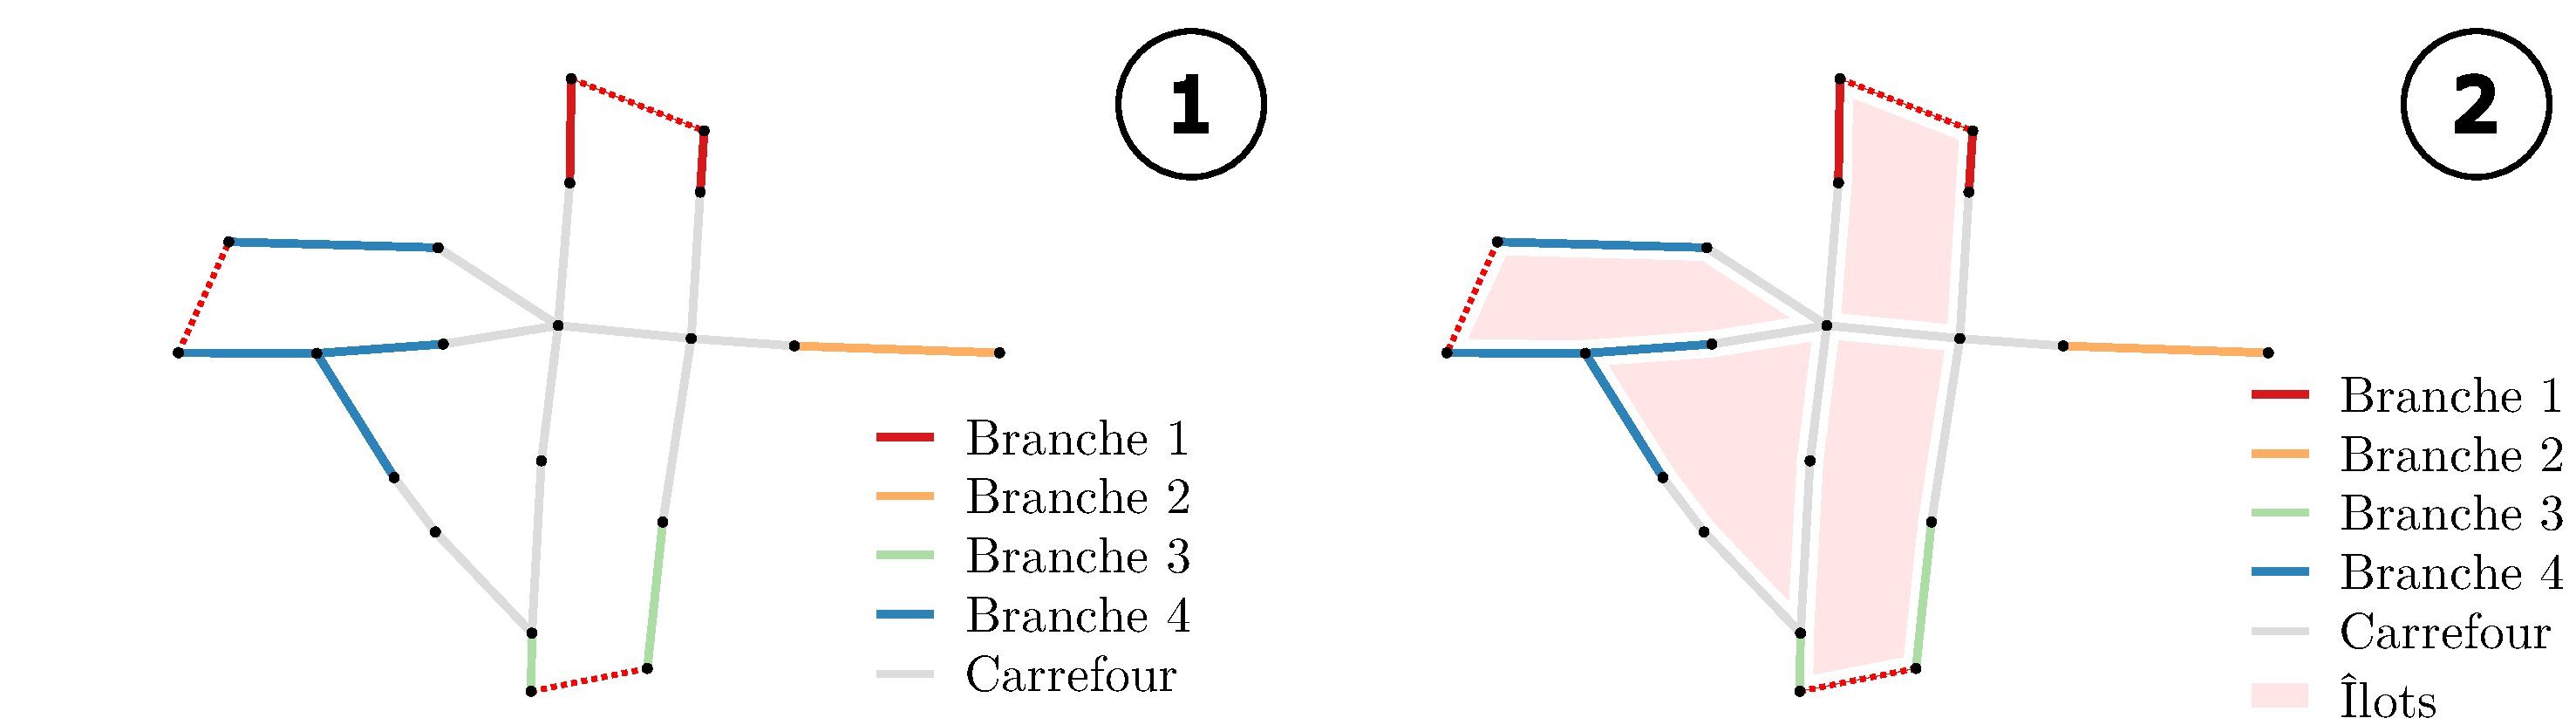
\includegraphics{images/modelisation/calcul_pieton/islands.pdf}}
    \caption{Étapes de génération des îlots. Source: \cite{Kalsron2022}.}
    \label{fig:modelisation_calcul_pieton_ilots}
\end{figure}

En dehors de la clé \osmkey{crossing:island} qui indique la présence d'un îlot au milieu d'une traversée mais dont la présence est marginale, les îlots sont absents de la sémantique d'\gls{osm}. En revanche, l'usage montre que les îlots sont représentés par les faces du graphe routier et peuvent être déduits de cette manière \cite{Vitalis2022}. Pour cela, il faut tout d'abord fermer les branches composées de plusieurs arêtes (voir figure \ref{fig:modelisation_calcul_pieton_ilots}.1) pour obtenir des faces et détecter l'intégralité des îlots (voir figure \ref{fig:modelisation_calcul_pieton_ilots}.2).

\subsubsection{Génération des traversées}

\begin{figure}
    \centering
    \resizebox{15cm}{!}{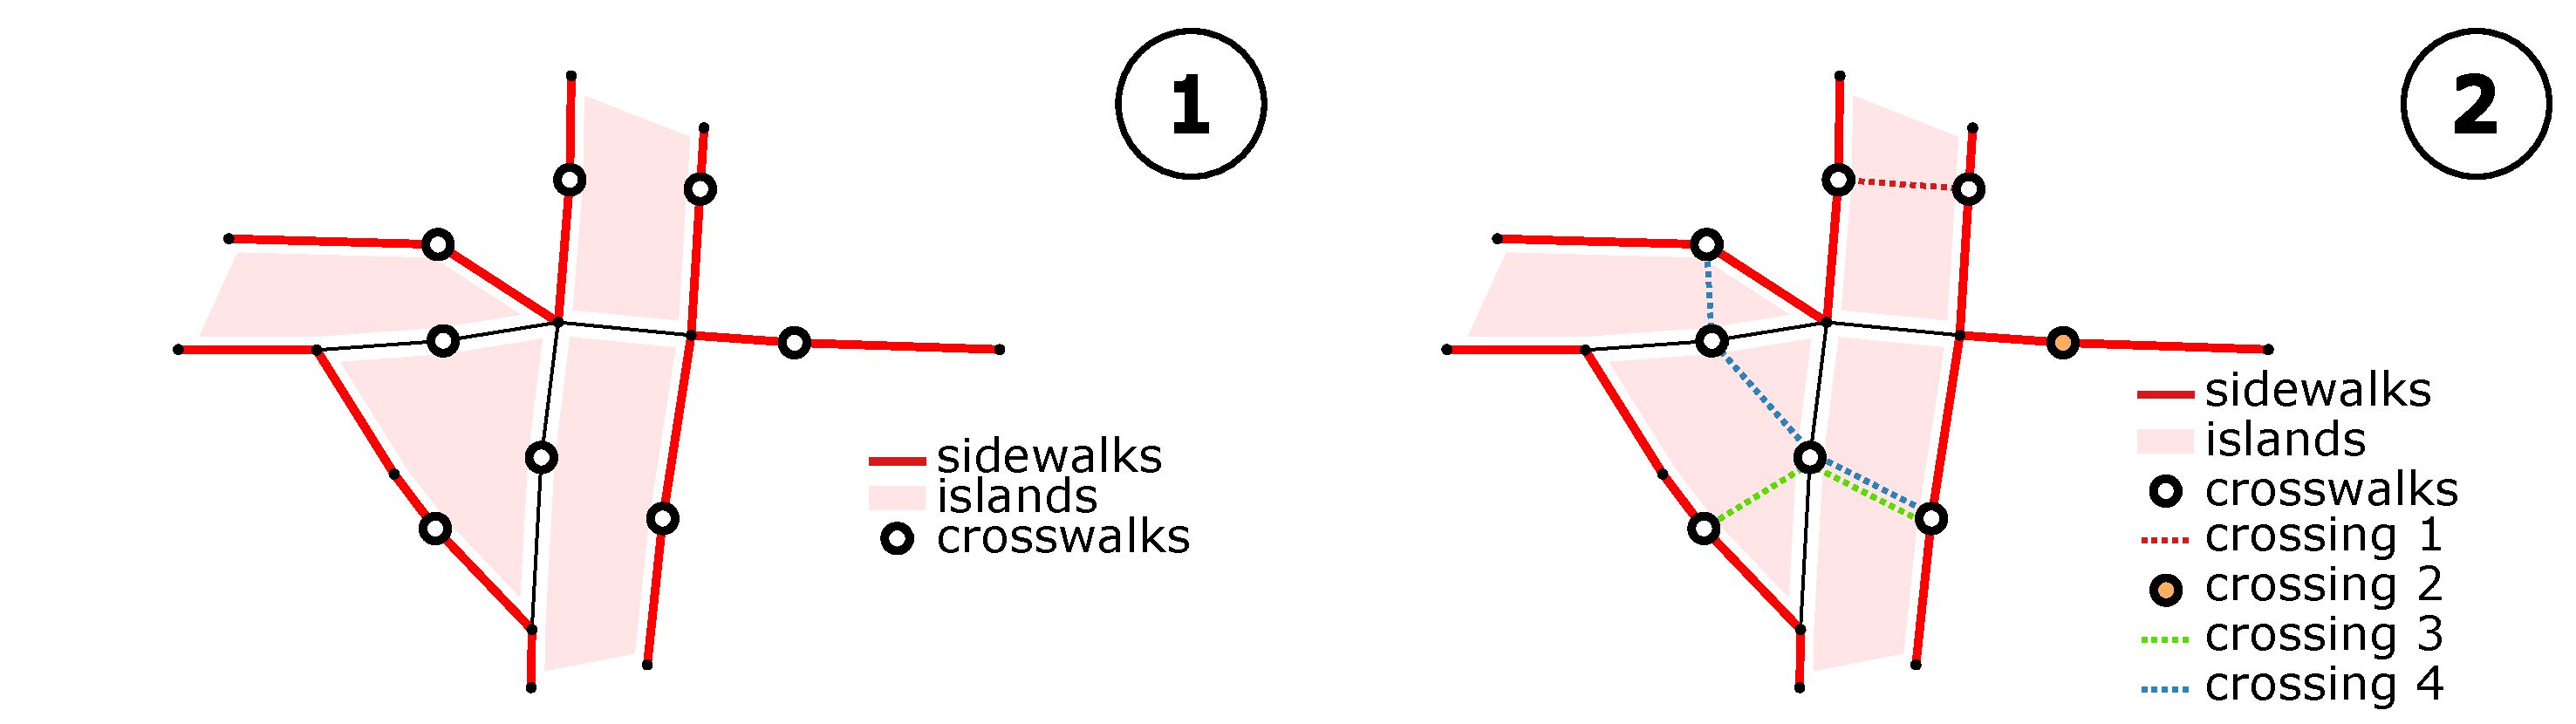
\includegraphics{images/modelisation/calcul_pieton/crossings.pdf}}
    \caption{Étapes de génération des traversées. Source: \cite{Kalsron2022}.}
    \label{fig:modelisation_calcul_pieton_traversees}
\end{figure}

Après avoir généré les trottoirs et les îlots, une traversée correspond à une séquence de passages piétons permettant de traverser d'un trottoir à un autre en passant uniquement par des îlots. On peut alors générer ces traversées en utilisant un graphe dual où les trottoirs et les îlots deviennent des nœuds, et les passages piétons des arêtes. Calculer les traversées revient alors à calculer le chemin le plus court entre deux trottoirs sans passer par un autre trottoir (voir figure \ref{fig:modelisation_calcul_pieton_traversees}).

\subsection{Construction de CrModel}

La construction de CrModel va correspondre à l'aggrégation des deux parties précédentes.

\todo{}